% !TeX spellcheck = es_ES

%----------------------------------------------------------------------------------------



\part{Capítulo tres}
\graphicspath{ {3_Capitulo/img/ejemplos/} {img/ch3/}, {W_Varios/2_Portada_capitulos} }

%----------------------------------------------------------------------------------------
%	CHAPTER 3
%----------------------------------------------------------------------------------------

\chapterimage{3_Capitulo/img/portada/ima2} % Chapter heading image
\chapter{Aplicaciones de interés compuesto}

\section{Mapa Mental}
\begin{center}
 \includegraphics[height = 5.6 cm]{3_Capitulo/img/explicacion/"Mapa Mental 3.pdf"}\\
\end{center}
\newpage
\section{Fórmulas del capítulo}
\begin{spacing}{1.5}
 \begin{center}
  \begin{tabular}{ |p{6cm}|p{7cm}| p{2cm}|}
   \hline
   \rowcolor{orange!50}
   \begin{center}\textbf{Fórmula} \end{center}             & \begin{center} \textbf{Nombre}\end{center} & \begin{center} \textbf{Excel} \end{center} \\ \hline
   $i =i_{1} + i_{2} + (i_{1})(  i_{2})$ & Tasas de referencia       & -                         \\ \hline
   $ i = \frac{i-i_{f}}{1+i_{f}} $       & Tasa de interés real      & -                         \\ \hline
  \end{tabular}
 \end{center}
\end{spacing}

\section{Depósito a término fijo}

Un intermediario financiero debe conseguir dinero del público con una tasa de interés que incentive a los inversionistas, esta tasa es llamada tasa de captación, para prestar este dinero con una tasa más alta llamada tasa de colocación.

\subsection{Certificado de depósito a término}
Es el certificado que se recibe por depósitos de sumas de dinero. Los plazos más usados son 30, 60, 90, 180 y 360 días. Pueden emitirlos las entidades financieras. La tasa de interés por su depósito está determinada por el monto, el plazo y las condiciones existentes en el mercado al momento de su constitución. Son nominativos y no se pueden redimir antes de su vencimiento.\\



%%%%%%%%%% NO OLVIDAR COLOCAR ESTE COMENTARIO CON EL NUMERO DE EJERCICIO %%%%%%%%%%%%%
%%%%%%%%%%%%%%%%%%% EJERCICIO 1 %%%%%%

\textbf{Ejemplo 1}\\
Una persona invierte 600{.}000  COP en un depósito a término fijo en 6 meses,a una tasa 24\%
nominal anual mes vencido, determinar la tasa efectiva anual y el valor del documento
suponiendo una retención en la fuente sobre utilidades del 7\%.\\ \\
%\newpage %USAR SOLO SI EL SOLUCIÓN QUEDA SOLO Y ES NECESARIO BAJARLO A LA SIGUIENTE PAGINA
\textbf{Solución.}\\
%La tabla ira centrada
\begin{center}
 \renewcommand{\arraystretch}{1.5}% Margenes de las celdas
 %Creación de la cuadricula de 3 columnas
 \begin{longtable}[H]{|c|c|c|}
  %Creamos una linea horizontal
  \hline
  \multicolumn{3}{|c|}{\cellcolor[HTML]{FFB183}\textbf{1. Asignación de periodo focal}}                                                                                                                \\ \hline
  \multicolumn{3}{|c|}{$pf = 6 \hspace{1mm} pmv$}                                                                                                                                      \\ \hline

  %Definimos el color de la primera fila
  \rowcolor[HTML]{FFB183}
  %%%%% INICIO DECLARACIÓN DE VARIABLES %%%%%%%
  %%%%%%%%%% INICIO TITULO
  %Lo que se hace aquí es mezclar las 3 columnas en una sola
  \multicolumn{3}{|c|}{\cellcolor[HTML]{FFB183}\textbf{2. Declaración de variables}}                                                                                                   \\ \hline
  %%%%%%%%%% FIN TITULO
  %%%%%%%%%% INICIO DE MATEMÁTICAS
  %Cada & hace referencia al paso de la siguiente columna
  $P =  600{.}000\ COP$                                                             & $m_{1} = 12 \textit{ pmv} $                                             & $F =  ? COP $                  \\
  $i= 2\% \textit{ pmv}$                                                       & $m_{2} = 1 \textit{ pmv} $                                              & $j_{2} = ?\% \textit{ naav} $ \\
  $n = 6  \textit{ pmv}  $                                                     & $j_ {1} = 24\% \textit{ namv} $                                         &                             \\
  $RF = 7\% \textit{ Retencion en la fuente}$                                  &                                                                         &                             \\\hline

  %%%%%%%%%% FIN DE MATEMÁTICAS
  %%%%% FIN DECLARACIÓN DE VARIABLES


  %%%%% INICIO FLUJO DE CAJA
  \rowcolor[HTML]{FFB183}
  \multicolumn{3}{|c|}{\cellcolor[HTML]{FFB183}\textbf{3. Diagrama de flujo de caja}}                                                                                                  \\ \hline
  %Mezclamos 3 columnas y pondremos el dibujo
  %%%%%%%%%%%%% INSERCIÓN DE LA IMAGEN
  %Deberán descargar las imágenes respectivas del drive y pegarlas en la carpeta
  %n_capitulo/img/ejemplos/1/capitulo1ejemplo1.pdf  (el /1/ es el numero del ejemplo)
  \multicolumn{3}{|c|}{ 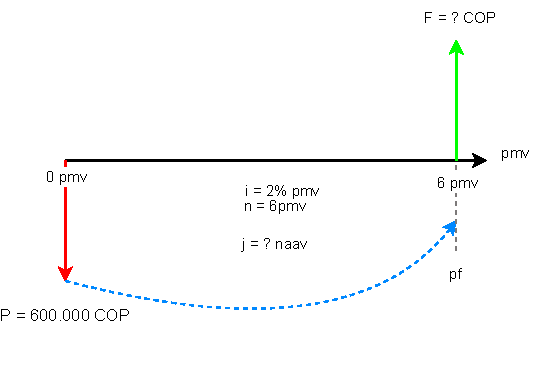
\includegraphics[trim=-78 -5 -78 -5]{3_Capitulo/img/ejemplos/1/capitulo3ejercicio1.pdf} }                                                                                      \\ \hline
  %%%%%%%%%%%%% FIN INSERCIÓN DE IMAGEN
  %%%%%FIN FLUJO DE CAJA



  %%%%% INICIO DECLARACIÓN FORMULAS
  %%%%%%%%%%% INICIO TITULO
  \rowcolor[HTML]{FFB183}
  \multicolumn{3}{|c|}{\cellcolor[HTML]{FFB183}\textbf{4. Declaración de Fórmulas}}                                                                                                    \\ \hline
  %%%%%%%%%%% FIN TITULO
  %%%%%%%%%%% INICIO MATEMÁTICAS

  $F = P(1+i)^n \hspace{0.3cm} \textit{Valor futuro}$                          & \multicolumn{2}{c|}{$(1+i_{1})^{m_{1}}=(1+i_{2})^{m_{2}}$  \textit{equivalencia de tasas}}                                            \\
  $j = i \cdot m \hspace{0.3cm} \textit{Tasa de interés periodica anualizada}$ & \multicolumn{2}{c|}{$I=F-P \hspace{0.3cm} \textit{Valor futuro neto}$}                                \\ \hline
  %%%%%%%%%% FIN MATEMÁTICAS
  %%%%%% INICIO DESARROLLO MATEMÁTICO
  \rowcolor[HTML]{FFB183}
  %%%%%%%%%%INICIO TITULO
  \multicolumn{3}{|c|}{\cellcolor[HTML]{FFB183}\textbf{5. Desarrollo Matemático}}                                                                                                      \\ \hline
  %%%%%%%%%% FIN TITULO
  %%%%%%%%%% INICIO MATEMÁTICAS
  $(1 + 0,02)^{12}= (1 + i_{2})^{1}$                                           & \multicolumn{2}{|c|}{$F =   600{.}000 \ COP \ (1+0,02)^6$}                                                     \\
  $i_{2}=(1+0,02)^{12}-1=0,26824179$                                           & \multicolumn{2}{|c|}{$F =  675{.}697,45 \ COP $}                                                            \\
  $j_{2}=0,26824179 \cdot 1 = 0,26824179\%naav$                                  & \multicolumn{2}{|c|}{$I = | F - P | = |   675.697,45 \ COP-  600.000 \ COP|$}                                  \\
  $j_{2}=26,824179\% \textit{ naav}$                                             & \multicolumn{2}{|c|}{$I = | F - P | = |  75.697,45  \ COP |$}                                               \\
  $j_{2}=26,48\% \cdot 1 = 26,48\% \textit{naav}$                                & \multicolumn{2}{|c|}{$RF = 0,07 \cdot  75{.}697,45 \ COP =  5{.}298,82 \ COP$}                                    \\
                                                                               & \multicolumn{2}{|c|}{$F_{final} =   675{.}697 \ COP-  5{.}299 \ COP =   670{.}398 \ COP$}                               \\ \hline


  %%%%%%%%%% FIN MATEMÁTICAS
  %%%%%% FIN DESARROLLO MATEMÁTICO
  %%%%%% INICIO RESPUESTA
  \rowcolor[HTML]{FFB183}
  %%%%%%%%%%INICIO TITULO
  \multicolumn{3}{|c|}{\cellcolor[HTML]{FFB183}\textbf{6. Respuesta}}                                                                                                                  \\ \hline
  %%%%%%%%%% FIN TITULO
  %%%%%%%%%% INICIO RESPUESTA MATEMÁTICA
  \multicolumn{3}{|p{\textwidth}|}{
  El valor del documento después de impuestos es de $ 670{.}398 \ COP$ que es menor que $F =  675{.}697,45 \ COP$ y obviamente se reduce la tasa de nominal anual mes vencido $j = 24,84\% \textit{ naav}$ .
  }                                                                                                                                                                                    \\ \hline


  %%%%%%%%%% FIN MATEMÁTICAS
  %%%%%% FIN RESPUESTA
 \end{longtable}
 %Se crean dos lineas en blanco para que no quede el siguiente texto tan pegado
 %\newline \newline %USARLO SI CREES QUE ES NECESARIO
\end{center}
%%%%%%%%%%%%%%%%%%%%%%%%%%FIN EJERCICIO 1 %%%%%%%%%%%%%%%%%%%%%%%%%%%


\subsection{Inflación ($i_f$)}
Mide el crecimiento del nivel general de precios de la economía. La inflación es calculada mensualmente por el DANE sobre los precios de una canasta básica de bienes y servicios de consumo para familias de ingresos medios y bajos. Con base en estos precios se calcula un índice denominado Índice de Precios al Consumidor (IPC). La inflación corresponde a la variación periódica de ese índice.\\
La inflación y la deflación son fenómenos internos de un país, la devaluación es externa.

\subsection{Índice}
Mide las variaciones de un fenómeno económico o de otro orden referido a un valor que se toma como base en un momento dado. Relación de precios, de cantidades, de valores entre dos períodos dados.

\subsection{Índice de precios al consumidor (IPC)}
Variación que entre un mes y otro presentan los precios de bienes y servicios de consumo final correspondientes a una canasta típica.

\subsection{Tasa promedio de captaciones Básica de Superfinanciera (TBS)}
Es la tasa promedio de captación a través de CDT y CDAT de las entidades financieras, calculada diariamente por la Superintendencia Financiera para diferentes plazos.

\section{Devaluación (idev)}
La pérdida de valor de una moneda frente a otra moneda se denomina devaluación (pagar  1{.}500 COP por un dólar,  2{.}000 COP un año después). En este caso la devaluación del año es igual a la variación de precio sobre el precio inicial, esto es: \\

devaluación = $\frac{ 2{.}000 \ COP - 1{.}500 \ COP}{ 1{.}500 \ COP} = 0,333333 $ = 33,33\% pav \\

La revaluación significa que habrá que pagar menos pesos por el mismo dólar (pagar  COP 1{.}500 por un dólar,  COP 1{.}200 un año después) entonces la revaluación será variación de precio sobre el precio inicial así: \\

revaluación = $\frac{ 1{.}200 \ COP - 1{.}500 \ COP}{ 1{.}500 \ COP} = -0,2$ = -20\% pav \\

\subsection{LIBOR (London Interbank Offer Rate)}
Tasa de interés anual para los préstamos interbancarios de primera clase en Londres y Europa.
\\
\\
%%%%%%%%%% NO OLVIDAR COLOCAR ESTE COMENTARIO CON EL NUMERO DE EJERCICIO %%%%%%%%%%%%%
%%%%%%%%%%%%%%%%%%% EJERCICIO 2 %%%%%%

\textbf{Ejemplo 2}\\
Un inversionista en Colombia adquiere un documento que vale 300 US, gana un
interés del 6\% nominal anual año vencido en dólares a un plazo de un año. El
tipo de cambio actual es  1 US =  1.500 COP y se estima una devaluación del peso con respecto al dólar durante ese año del 20\% efectivo anual. Calcular la rentabilidad que se podía obtener. ¿Cuál es la rentabilidad neta, una vez descontada la retención en la fuente del 7\%?\\ \\
%\newpage %USAR SOLO SI EL SOLUCIÓN QUEDA SOLO Y ES NECESARIO BAJARLO A LA SIGUIENTE PAGINA
\textbf{Solución.}\\
%La tabla ira centrada
\begin{center}
 \renewcommand{\arraystretch}{1.5}% Margenes de las celdas
 %Creación de la cuadricula de 3 columnas
 \begin{longtable}[H]{|c|c|c|}
  %Creamos una linea horizontal
  \hline
  %Definimos el color de la primera fila
  \rowcolor[HTML]{FFB183}
  %%%%% INICIO DECLARACIÓN DE VARIABLES %%%%%%%
  %%%%%%%%%% INICIO TITULO
  %Lo que se hace aquí es mezclar las 3 columnas en una sola
\multicolumn{3}{|c|}{\cellcolor[HTML]{FFB183}\textbf{1. Asignación de Periodo Focal}}                                        \\ \hline
  %%%%%%%%%% FIN TITULO
  %%%%%%%%%% INICIO DE MATEMÁTICAS
  %Cada & hace referencia al paso de la siguiente columna
  \multicolumn{3}{|c|}{\textit{$pf = 1 pav$}}                                                            \\ \hline
  \multicolumn{3}{|c|}{\cellcolor[HTML]{FFB183}\textbf{2. Declaración de variables}}                                        \\ \hline
  %%%%%%%%%% FIN TITULO
  %%%%%%%%%% INICIO DE MATEMÁTICAS
  %Cada & hace referencia al paso de la siguiente columna
  $j = 6\% \textit{ naav en US}$                                     & $n = 1 \textit{ pav} $ & $j_{dev}=20\% \textit{ naav}$ \\
  $i = \frac{6 \textit{ naav}}{1 \textit{ pav}} = 6\% \textit{ pav}$ & dólar:1 US = $ 1.500 \ COP $  &                             \\ \hline

  %%%%%%%%%% FIN DE MATEMÁTICAS
  %%%%% FIN DECLARACIÓN DE VARIABLES


  %%%%% INICIO FLUJO DE CAJA
  \rowcolor[HTML]{FFB183}
  \multicolumn{3}{|c|}{\cellcolor[HTML]{FFB183}\textbf{3. Diagrama de flujo de caja}}                                       \\ \hline
  %Mezclamos 3 columnas y pondremos el dibujo
  %%%%%%%%%%%%% INSERCIÓN DE LA IMAGEN
  %Deberán descargar las imágenes respectivas del drive y pegarlas en la carpeta
  %n_capitulo/img/ejemplos/1/capitulo1ejemplo1.pdf  (el /1/ es el numero del ejemplo)
  \multicolumn{3}{|c|}{ 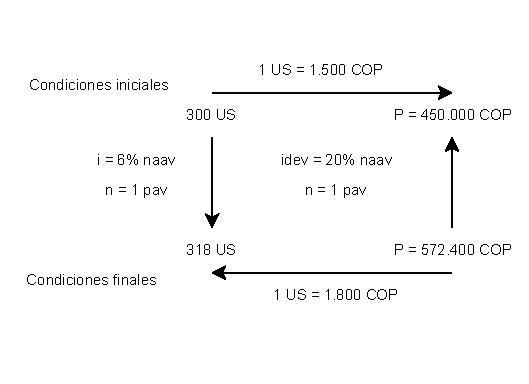
\includegraphics[trim=-78 -5 -78 -5]{3_Capitulo/img/ejemplos/2/capitulo3ejercicio2.pdf} }                         \\ \hline
  %%%%%%%%%%%%% FIN INSERCIÓN DE IMAGEN
  %%%%%FIN FLUJO DE CAJA



  %%%%% INICIO DECLARACIÓN FORMULAS
  %%%%%%%%%%% INICIO TITULO
  \rowcolor[HTML]{FFB183}
  \multicolumn{3}{|c|}{\cellcolor[HTML]{FFB183}\textbf{4. Declaración de Fórmulas}}                                         \\ \hline
  %%%%%%%%%%% FIN TITULO
  %%%%%%%%%%% INICIO MATEMÁTICAS
  \multicolumn{3}{|c|}{$F = P (1 + i)^n \textit{ Valor futuro}$}                                                            \\ \hline
  %%%%%%%%%% FIN MATEMÁTICAS
  %%%%%% INICIO DESARROLLO MATEMÁTICO
  \rowcolor[HTML]{FFB183}
  %%%%%%%%%%INICIO TITULO
  \multicolumn{3}{|c|}{\cellcolor[HTML]{FFB183}\textbf{5. Desarrollo Matemático}}                                           \\ \hline
  %%%%%%%%%% FIN TITULO
  %%%%%%%%%% INICIO MATEMÁTICAS
    \multicolumn{3}{|p{\textwidth}|}{
  $300 \ US$ en pesos, $(300)1{.}500 =  450{.}000 \ COP$ \vspace{3mm} \newline

  $F = 300 \ US(1 + 0,06)1 = 318 \ US$ \vspace{3mm} \newline

  $F =  1{.}500 \ COP (1 + 0,02)^1=  1{.}800 \ COP$\newline

  $  (318 \ US)\frac{ 1{.}800 \ COP}{1 \ US}= 572{.}400 \ COP$\newline

  $ \frac{(318 US \  COP) 1{.}800 \ COP}{ 1 \ US} =  572{.}400 \ COP$ \newline
  }                                                                                                                         \\ \hline
\multicolumn{3}{|c|}{\cellcolor[HTML]{FFB183}\textbf{6. Respuesta}}                                         \\ \hline
  %%%%%%%%%%% FIN TITULO
  %%%%%%%%%%% INICIO MATEMÁTICAS
\multicolumn{3}{|p{\textwidth}|}{El valor de la rentabilidad sin descontar la retención en la fuente era de 572.400 COP con un i del 27,2\%. Al descontar la retención en la fuente esa rentabilidad neta es de
563,832 COP, con un i del 25\%}  \\ \hline
  %%%%%%%%%% FIN MATEMÁTICAS

  %%%%%%%%%% FIN MATEMÁTICAS
  %%%%%% FIN DESARROLLO MATEMÁTICO
  %%%%%% INICIO RESPUESTA



  %%%%%%%%%% FIN MATEMÁTICAS
  %%%%%% FIN RESPUESTA
 \end{longtable}
 %Se crean dos lineas en blanco para que no quede el siguiente texto tan pegado
 %\newline \newline %USARLO SI CREES QUE ES NECESARIO
\end{center}
%%%%%%%%%%%%%%%%%%%%%%%%%%FIN EJERCICIO 2 %%%%%%%%%%%%%%%%%%%%%%%%%%%


\section{Tasas combinadas}

Cuando se combina una tasa $i_{1}$ con una tasa $i_{2}$, con el objetivo de facilitar los cálculos se puede utilizar la tasa combinada "i". Para este fin se usa la siguiente fórmula:\\
\centerline{$ i = i_{1} +i_{2} + (i_{1})( i_{2})$ \hspace{15pt}\textit{ Tasas combinadas}\\}
\textbf{Nota:} Se utiliza únicamente para el cálculo de tasas de interés anuales, por ejemplo, para calcular la tasa equivalente entre dos tasas efectivas.\\


%%%%%%%%%% NO OLVIDAR COLOCAR ESTE COMENTARIO CON EL NUMERO DE EJERCICIO %%%%%%%%%%%%%
%%%%%%%%%%%%%%%%%%% EJERCICIO 3 %%%%%%
\newpage
\textbf{Ejemplo 3}\\
Resolver el ejemplo 2 usando la tasa combinada.\\ \\
%\newpage %USAR SOLO SI EL SOLUCIÓN QUEDA SOLO Y ES NECESARIO BAJARLO A LA SIGUIENTE PAGINA
\textbf{Solución.}\\
%La tabla ira centrada
\begin{center}
 \renewcommand{\arraystretch}{1.5}% Margenes de las celdas
 %Creación de la cuadricula de 3 columnas
 \begin{longtable}[H]{|c|c|c|}
  %Creamos una linea horizontal
  \hline
  %Definimos el color de la primera fila
  \rowcolor[HTML]{FFB183}
  %%%%% INICIO DECLARACIÓN DE VARIABLES %%%%%%%
  %%%%%%%%%% INICIO TITULO
  \multicolumn{3}{|c|}{\cellcolor[HTML]{FFB183}\textbf{1. Asignación período focal}}                                                    \\ \hline
  \multicolumn{3}{|c|}{$pf=1\textit{ pav}$}                                                                                            \\ \hline
  %Lo que se hace aquí es mezclar las 3 columnas en una sola
  \multicolumn{3}{|c|}{\cellcolor[HTML]{FFB183}\textbf{2. Declaración de variables}}                \\ \hline
  %%%%%%%%%% FIN TITULO
  %%%%%%%%%% INICIO DE MATEMÁTICAS
  %Cada & hace referencia al paso de la siguiente columna
  \multicolumn{3}{|c|}{$j_{1} = 6\% \textit{ naav en US}$}                                         \\
  \multicolumn{3}{|c|}{$j_{2} = 20\% \textit{ naav en COL}$}                                        \\ \hline

  %%%%%%%%%% FIN DE MATEMÁTICAS
  %%%%% FIN DECLARACIÓN DE VARIABLES


  %%%%% INICIO FLUJO DE CAJA
  \rowcolor[HTML]{FFB183}
  \multicolumn{3}{|c|}{\cellcolor[HTML]{FFB183}\textbf{3. Diagrama de flujo de caja}}               \\ \hline
  %Mezclamos 3 columnas y pondremos el dibujo
  %%%%%%%%%%%%% INSERCIÓN DE LA IMAGEN
  %Deberán descargar las imágenes respectivas del drive y pegarlas en la carpeta
  %n_capitulo/img/ejemplos/1/capitulo1ejemplo1.pdf  (el /1/ es el numero del ejemplo)
  \multicolumn{3}{|c|}{ 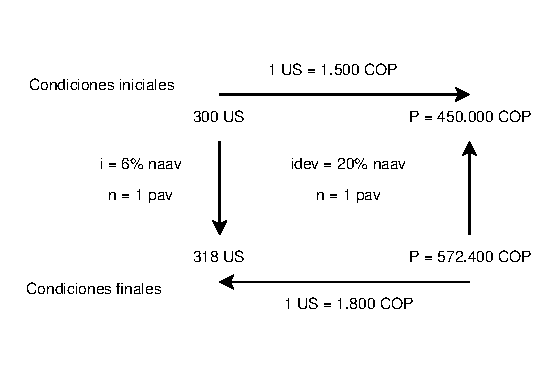
\includegraphics[trim=-78 -5 -78 -5]{3_Capitulo/img/ejemplos/3/capitulo3ejercicio3.pdf} }  \\ \hline
  %%%%%%%%%%%%% FIN INSERCIÓN DE IMAGEN
  %%%%%FIN FLUJO DE CAJA



  %%%%% INICIO DECLARACIÓN FORMULAS
  %%%%%%%%%%% INICIO TITULO
  \rowcolor[HTML]{FFB183}
  \multicolumn{3}{|c|}{\cellcolor[HTML]{FFB183}\textbf{4. Declaración de Fórmulas}}                 \\ \hline
  %%%%%%%%%%% FIN TITULO
  %%%%%%%%%%% INICIO MATEMÁTICAS

  \multicolumn{3}{|c|}{$i = i_{1}+i_{2}+i_{1}\cdot i{2}  \hspace{1cm}\textit{ Tasas combinadas}$}   \\
  \multicolumn{3}{|c|}{$j = i \cdot m \hspace{1cm}\textit{ Tasa periódica anualizada}$}             \\ \hline
  %%%%%%%%%% FIN MATEMÁTICAS
  %%%%%% INICIO DESARROLLO MATEMÁTICO
  \rowcolor[HTML]{FFB183}
  %%%%%%%%%%INICIO TITULO
  \multicolumn{3}{|c|}{\cellcolor[HTML]{FFB183}\textbf{5. Desarrollo Matemático}}                   \\ \hline
  %%%%%%%%%% FIN TITULO
  %%%%%%%%%% INICIO MATEMÁTICAS
  \multicolumn{3}{|l|}{$i_{1} = \frac{6\% \textit{ naav}}{1}= 6\% \textit{ pav}$}                   \\
  \multicolumn{3}{|l|}{$i_{2} = \frac{20\% \textit{ naav}}{1}= 20\% \textit{pav}$}                  \\
  \multicolumn{3}{|l|}{$i = 0,06+0,2+0,06 \cdot 0,2 = 0,272 \textit{ pav} \equiv i = 27,2\% \textit{ pav}$}                \\
  \multicolumn{3}{|l|}{$j = 27,2\% \cdot 1 = 27,2\% \textit{ naav}$}                                \\ \hline



  %%%%%%%%%% FIN MATEMÁTICAS
  %%%%%% FIN DESARROLLO MATEMÁTICO
  %%%%%% INICIO RESPUESTA
  \rowcolor[HTML]{FFB183}
  %%%%%%%%%%INICIO TITULO
  \multicolumn{3}{|c|}{\cellcolor[HTML]{FFB183}\textbf{6. Respuesta}}                               \\ \hline
  %%%%%%%%%% FIN TITULO
  %%%%%%%%%% INICIO RESPUESTA MATEMÁTICA
\multicolumn{3}{|c|}{$j=27,2\%\textit{ naav}$}                                                                                                \\ \hline


  %%%%%%%%%% FIN MATEMÁTICAS
  %%%%%% FIN RESPUESTA
 \end{longtable}

 %Se crean dos lineas en blanco para que no quede el siguiente texto tan pegado
 %\newline \newline %USARLO SI CREES QUE ES NECESARIO
\end{center}
%%%%%%%%%%%%%%%%%%%%%%%%%%FIN EJERCICIO 3 %%%%%%%%%%%%%%%%%%%%%%%%%%%



\section{Tasa real}
Para un proyecto de inversión se tiene en cuenta que la inflación afecta la rentabilidad real del proyecto y que siempre se desea obtener una rentabilidad superior a la tasa de oportunidad. Para calcular la rentabilidad real se hace uso de la fórmula asumiendo que la inflación "$i_{1} = i_ {f} $", que la rentabilidad "$i_{2} = i_ {R} $" y que la rentabilidad que en total paga es "i", por tanto se tiene y despejando "$i_{R}$" de:
\begin{align*}
 i= i_{f} + i_{R} + i_{f} i_{R}
\end{align*}
\begin{align*}
 i_{R} = \frac{i-i_{f}}{1+i_{f}}\hspace{35pt}\textit{ Tasa de interés real}
\end{align*}



%%%%%%%%%% NO OLVIDAR COLOCAR ESTE COMENTARIO CON EL NUMERO DE EJERCICIO %%%%%%%%%%%%%
%%%%%%%%%%%%%%%%%%% EJERCICIO 4 %%%%%%

\textbf{Ejemplo 4}\\
Calcular la rentabilidad que gana el inversionista del ejemplo 2 teniendo
en cuenta que la inflación para el año en el que se hizo la inversión fue del
18\% efectivo anual. ¿Cuál es la rentabilidad neta una vez descontada la
retención en la fuente y la inflación?\\ \\
%\newpage %USAR SOLO SI EL SOLUCIÓN QUEDA SOLO Y ES NECESARIO BAJARLO A LA SIGUIENTE PAGINA
\textbf{Solución.}\\
%La tabla ira centrada
\begin{center}
 \renewcommand{\arraystretch}{1.5}% Margenes de las celdas
 %Creación de la cuadricula de 3 columnas
 \begin{longtable}[H]{|c|c|c|}
  %Creamos una linea horizontal
  \hline
  %Definimos el color de la primera fila
  \rowcolor[HTML]{FFB183}
  \multicolumn{3}{|c|}{\cellcolor[HTML]{FFB183}\textbf{1. Asignación período focal}}                                                    \\ \hline
  \multicolumn{3}{|c|}{$pf=1\textit{pav}$}                                                                                            \\ \hline


  %%%%% INICIO DECLARACIÓN DE VARIABLES %%%%%%%
  %%%%%%%%%% INICIO TITULO
  %Lo que se hace aquí es mezclar las 3 columnas en una sola
  \multicolumn{3}{|c|}{\cellcolor[HTML]{FFB183}\textbf{2. Declaración de variables}}                                                  \\ \hline
  %%%%%%%%%% FIN TITULO
  %%%%%%%%%% INICIO DE MATEMÁTICAS
  %Cada & hace referencia al paso de la siguiente columna
  %Cada & hace referencia al paso de la siguiente columna
  \multicolumn{2}{|l|}{ $i = 27,2\% \textit{pav}$ }                                   & $i_{R}=?$                                     \\
  \multicolumn{2}{|l|}{$i_{f} = 18\% \textit{ naav}=18\% \textit{ naav}$  }           &                                               \\
  \multicolumn{2}{|l|}{$i_{f} = \frac{18\%}{1}\textit{naav }=18\%  \textit{naav }$  } &                                               \\ \hline

  %%%%%%%%%% FIN DE MATEMÁTICAS
  %%%%% FIN DECLARACIÓN DE VARIABLES


  %%%%% INICIO FLUJO DE CAJA
  \rowcolor[HTML]{FFB183}
  \multicolumn{3}{|c|}{\cellcolor[HTML]{FFB183}\textbf{3. Diagrama de flujo de caja}}                                                 \\ \hline
  %Mezclamos 3 columnas y pondremos el dibujo
  %%%%%%%%%%%%% INSERCIÓN DE LA IMAGEN
  %Deberán descargar las imágenes respectivas del drive y pegarlas en la carpeta
  %n_capitulo/img/ejemplos/1/capitulo1ejemplo1.pdf  (el /1/ es el numero del ejemplo)
  \multicolumn{3}{|c|}{ 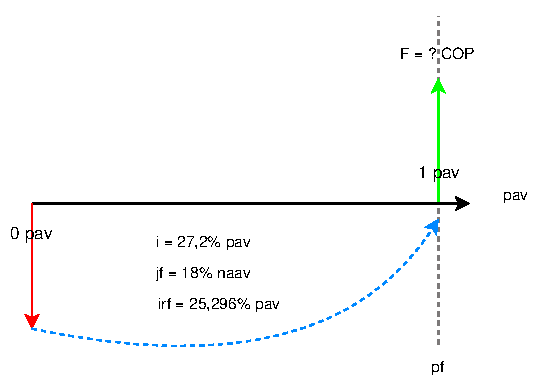
\includegraphics[trim=-78 -5 -78 -5]{3_Capitulo/img/ejemplos/4/capitulo3ejercicio4.pdf} }                                    \\ \hline
  %%%%%%%%%%%%% FIN INSERCIÓN DE IMAGEN
  %%%%%FIN FLUJO DE CAJA



  %%%%% INICIO DECLARACIÓN FORMULAS
  %%%%%%%%%%% INICIO TITULO
  \rowcolor[HTML]{FFB183}
  \multicolumn{3}{|c|}{\cellcolor[HTML]{FFB183}\textbf{4. Declaración de Fórmulas}}                                                   \\ \hline
  %%%%%%%%%%% FIN TITULO
  %%%%%%%%%%% INICIO MATEMÁTICAS

  \multicolumn{3}{|c|}{$i_{R}=\frac{i-i_{f}}{1+i_{f}}$\hspace{2mm} Tasa de interés real }                                             \\ \hline
  %%%%%%%%%% FIN MATEMÁTICAS
  %%%%%% INICIO DESARROLLO MATEMÁTICO
  \rowcolor[HTML]{FFB183}
  %%%%%%%%%%INICIO TITULO
  \multicolumn{3}{|c|}{\cellcolor[HTML]{FFB183}\textbf{5. Desarrollo Matemático}}                                                     \\ \hline
  %%%%%%%%%% FIN TITULO
  %%%%%%%%%% INICIO MATEMÁTICAS
  \multicolumn{3}{|p{\textwidth}|}{$i_{R} =0,272-0,181+0,18= 0,077966 = 7,8\% \textit{ pav}$}                                         \\
  \multicolumn{3}{|p{\textwidth}|}{$i_{R} = \frac{(0,25296 - 0,18)}{(1 + 0,18)} \textit{ Tasa de interes de retencion en la fuente}$} \\
  \multicolumn{3}{|p{\textwidth}|}{$i_{R} = 6,18305085\% \textit{ pav}$}                                                              \\
  \multicolumn{3}{|p{\textwidth}|}{$j_{R} = 6,18305085\% \textit{naav}$}                                                                \\ \hline

  %%%%%%%%%% FIN MATEMÁTICAS
  %%%%%% FIN DESARROLLO MATEMÁTICO


  %%%%%%%%%% FIN MATEMÁTICAS
  %%%%%% FIN RESPUESTA
 \end{longtable}
 %Se crean dos lineas en blanco para que no quede el siguiente texto tan pegado
 %\newline \newline %USARLO SI CREES QUE ES NECESARIO
\end{center}
%%%%%%%%%%%%%%%%%%%%%%%%%%FIN EJERCICIO 4 %%%%%%%%%%%%%%%%%%%%%%%%%%%



\section{Tasas combinadas}
Hay muchos créditos atados a una tasa principal, por ejemplo a la inflación más unos puntos adicionales, estos puntos adicionales se denomina el spread, suponiendo que la inflación fuera del 10\% efectivo anual y que el spread sea de 5 puntos, entonces la tasa a la cual se cancelará el crédito se puede calcular aplicando la fórmula de las tasas combinadas: \\

$i= 0,1 pav + 0,05 pav + 0,1 x 0,05 = 0,155 pav \equiv 15,5\% pav  \rightarrow  j = 15,5\% pav x1 pav = 15,5\%naav \equiv 15,5 \%naav$ \\

Cuando la tasa principal viene dada en forma efectivo anual para agregarle el spread se usa la fórmula de combinación de tasas, pero si el spread se le adiciona a una tasa nominal entonces el spread simplemente se suma a la tasa principal, por ejemplo: \\

Si un préstamo para vivienda se otorga a la tasa de los depósitos a término fijo-DTF (tasa principal) más 8 puntos y suponiendo que la tasa de depósito a término fijo -DTF lo mismo que la sea del 17\% nominal anual trimestre anticipado, entonces la tasa del crédito será: \\

$i = i_{1} + i_{2}
 i = 17\%nata + 8\%nata = 25\% nata$\\\\ Las tasas equivalente nominales se suma en igual período y modalidad, en tasas efectivas anuales se aplica la equivalencia de tasas de referencia.Por equivalencia de tasas se concluye que es equivalente al 29,45\% efectivo anual.\\

\textbf{Observación:} Para créditos es costumbre que la tasa de depósito a término fijo -DTF lo mismo que la tasa de captación de las corporaciones-TCC se expresan en nominal anual trimestre anticipado y en tasa de captación de la tasa de depósito a término fijo -DTF y de la tasa de captación de las corporaciones-TCC se expresa en efectivo anual.\\



%%%%%%%%%% NO OLVIDAR COLOCAR ESTE COMENTARIO CON EL NUMERO DE EJERCICIO %%%%%%%%%%%%%
%%%%%%%%%%%%%%%%%%% EJERCICIO 5 %%%%%%
\newpage
\textbf{Ejemplo 5}\\
Una persona tiene un préstamo hipotecario al IPC + 4 puntos ¿Cuál
debe ser el spread si se cambia a otro plan cuya tasa es la DTF +X?
Suponga que el IPC = 8\% efectiva anual y que la DTF = 18,67\% nominal
anual trimestre anticipado, en donde IPC: Tasa del Índice de Precios al
Consumidor DTF: Tasa de Depósito a Término Fijo promedio.\\ \\
%\newpage %USAR SOLO SI EL SOLUCIÓN QUEDA SOLO Y ES NECESARIO BAJARLO A LA SIGUIENTE PAGINA
\textbf{Solución.}\\
%La tabla ira centrada
\begin{center}
 \renewcommand{\arraystretch}{1.5}% Margenes de las celdas
 %Creación de la cuadricula de 3 columnas
 \begin{longtable}[H]{|p{0.3750\linewidth}|p{0.3750\linewidth}|p{0.25\linewidth}|}
  %Creamos una linea horizontal
  \hline
  %Definimos el color de la primera fila
  \rowcolor[HTML]{FFB183}
  %%%%% INICIO ASIGNACIÓN FECHA FOCAL %%%%%%%
  %%%%%%%%%% INICIO TITULO
  %Lo que se hace aquí es mezclar las 3 columnas en una sola
  \multicolumn{3}{|c|}{\cellcolor[HTML]{FFB183}\textbf{1. Asignación período focal}}                                                                \\ \hline
  %%%%%%%%%% FIN TITULO
  \multicolumn{3}{|c|}{  $pf = 1 \textit{ pav} = 4 \textit{ ptv}$}                                                                                \\ \hline

  %%%%% INICIO DECLARACIÓN DE VARIABLES %%%%%%%
  %%%%%%%%%% INICIO TITULO
  %Lo que se hace aquí es mezclar las 3 columnas en una sola
  \multicolumn{3}{|c|}{\cellcolor[HTML]{FFB183}\textbf{2. Declaración de variables}}                                                              \\ \hline
  %%%%%%%%%% FIN TITULO
  %%%%%%%%%% INICIO DE MATEMÁTICAS
  %Cada & hace referencia al paso de la siguiente columna
  $j_{1} = 8\% \textit{ naav}$     & $m_{1} = 1 \textit{ naav} $ & $X = ? \% $                                                                       \\
  $j_{2} = 18,67\% \textit{ nata}$ & $m_{2} = 4 \textit{ ptv} $  &                                                                                \\ &                             & \\ & 				           					 & 	 \\ \hline

  %%%%%%%%%% FIN DE MATEMÁTICAS
  %%%%% FIN DECLARACIÓN DE VARIABLES


  %%%%% INICIO DECLARACIÓN FORMULAS
  %%%%%%%%%%% INICIO TITULO
  \rowcolor[HTML]{FFB183}
  \multicolumn{3}{|c|}{\cellcolor[HTML]{FFB183}\textbf{3. Declaración de fórmulas}}                                                               \\ \hline
  %%%%%%%%%%% FIN TITULO
  %%%%%%%%%%% INICIO MATEMÁTICAS
  \multicolumn{3}{|l|}{$IPC + 4 = DTF + X \hspace{1cm}\textit{Ecuación de valor}$}                                                                \\
  \multicolumn{3}{|l|}{$i = i_{1} + i_{2} + (i_{1})(i_{2})\hspace{1cm}\textit{Tasas combinadas}$}                                                 \\

  \multicolumn{3}{|l|}{$i_{a} =i_{1} + i \hspace{3cm}\textit{Tasa de interés períodica anticipada}$}                                              \\
  \multicolumn{3}{|l|}{$ (1 + i_{1})\cdot m_{1} = (1 + i2)\cdot m_{2} \hspace{1cm}\textit{Equivalencia tasas anticipadas}$}                       \\
  \multicolumn{3}{|l|}{$ j_{a} = i_{m} \hspace{1cm}\textit{Tasa nominal anual}$}                                                                  \\
  \multicolumn{3}{|l|}{$\textit{Tasa del crédito} = IPC + 4 \textit{ puntos efectivos anuales} = DTF + x( \textit{ spread en}\% \textit{ nata})$} \\ \hline

  %%%%%%%%%% FIN MATEMÁTICAS
  %%%%%% INICIO DESARROLLO MATEMÁTICO
  \rowcolor[HTML]{FFB183}
  %%%%%%%%%%INICIO TITULO
  \multicolumn{3}{|c|}{\cellcolor[HTML]{FFB183}\textbf{5. Desarrollo matemático}}                                                                 \\ \hline
  %%%%%%%%%% FIN TITULO
  %%%%%%%%%% INICIO MATEMÁTICAS
  \multicolumn{3}{|p{\textwidth}|}{
  Calcularemos la tasa neta del crédito inicial que está en naav, a partir de la fórmula de tasas
  combinadas, las fórmulas interés periódica vencida y luego la tasa periódica trimestre
  anticipada, para luego igualar la tasa nominal anual trimestre anticipada y despejar la X=?
  nata.\newline
  \setlength{\parskip}{0.1mm}

  $IPC + 4 = 0,08 + 0,04 + 0,08 \cdot 0,04$\newline

  $\textit{Tasa del crédito} = IPC + 4 \textit{ puntos}$\newline

  $\textit{Tasa de crédito inicial} = 0,08 + 0,04 + 0,08 \cdot 0,04 \textit{ naav}$\newline

  $IPC + 4 = 12,32\%\textit{ pav equivalente a} 12,32\%\textit{ naav}$\newline

  $(1 + 0,1232)^1 = (1 + i)^4$\newline

  $i = 2,947137112\%\textit{ ptv}$\newline

  $i_{a} =\frac{0,02947137112}{1 + 0,02947137112} = 0,0286275\%\textit{ pta}$\newline

  $ja = 2,86875  \cdot  4 = 11,451\%\textit{ nata}$\newline

  $\textit{Tasa de crédito equivalente} = DTF + X(\%\textit{ nata})$\newline

  $\textit{Tasa de crédito equivalente} = 11,45\% \textit{ nata} = 18,67\% \textit{ nata} + X\%\textit{ nata}$\newline

  $\textit{Entonces } X = 11,451\% \textit{ nata} - 12,32\% \textit{ nata} = -7,219\%nata$\newline

  $DTF + X = 0,1867 + X \textit{ nata}$\newline

  $0,11451 = 0,1867 + \textit{ nata donde X}   = -0,07219$\newline

  $X = -7,219\% \textit{ nata}$\newline
  \setlength{\parskip}{0mm}
  }                                                                                                                                               \\ \hline


  %%%%%%%%%% FIN MATEMÁTICAS
  %%%%%% FIN DESARROLLO MATEMÁTICO
  %%%%%% INICIO RESPUESTA
  \rowcolor[HTML]{FFB183}
  %%%%%%%%%%INICIO TITULO
  \multicolumn{3}{|c|}{\cellcolor[HTML]{FFB183}\textbf{6. Respuesta}}                                                                             \\ \hline
  %%%%%%%%%% FIN TITULO
  %%%%%%%%%% INICIO RESPUESTA MATEMÁTICA
  \multicolumn{3}{|C{\textwidth}|}{
  $X = -7,219\% \textit{nata}$
  }                                                                                                                                               \\ \hline


  %%%%%%%%%% FIN MATEMÁTICAS
  %%%%%% FIN RESPUESTA
 \end{longtable}
 %Se crean dos lineas en blanco para que no quede el siguiente texto tan pegado
 %\newline \newline %USARLO SI CREES QUE ES NECESARIO
\end{center}
%%%%%%%%%%%%%%%%%%%%%%%%%%FIN EJERCICIO 5 %%%%%%%%%%%%%%%%%%%%%%%%%%%

%\textbf{Observación 1:} En Colombia el spread se da en puntos que son adicionales a la tasa principal, en Europa y Estados Unidos el spread se acostumbra a dar en puntos básicos. Un punto básico es igual al 0,01\% de forma que 400 puntos básicos corresponden a un spread de 4 puntos.\\
%
%\textbf{Observación 2:} A pesar de que la Libor es una tasa efectiva, es costumbre que el spread simplemente se sume a la Libor sin hacer uso de la tasa combinada, La razón es que éstas tasas son muy pequeñas y la diferencia de resultados entre un método y otro es prácticamente nula.\\

%%%%%%%%%% NO OLVIDAR COLOCAR ESTE COMENTARIO CON EL NUMERO DE EJERCICIO %%%%%%%%%%%%%
%%%%%%%%%%%%%%%%%%% EJERCICIO 6 %%%%%%
\newpage
\textbf{Ejemplo 6}\\
Una industria tiene actualmente contratado un préstamo con una
corporación financiera a la tasa del TCC+3 puntos. ¿Cuál debe ser el spread
en puntos básicos de forma tal que financiera mente sea indiferente el
préstamo en la corporación financiera o en el mercado de Londres? con
estos índices:\\ \\
\begin{itemize}
 \item $TCC = 15,3\% \textit{ nata}$
 \item $i_{dev} = 22\% \textit{ naav}$
\end{itemize}
Interés devaluación del peso Colombiano con respecto a la libra esterlina Libor
\begin{itemize}
 \item  $Libor= 5,2\% \textit{ naav}$. Tasa de interés del mercado europeo
\end{itemize}
%\newpage %USAR SOLO SI EL SOLUCIÓN QUEDA SOLO Y ES NECESARIO BAJARLO A LA SIGUIENTE PAGINA
\textbf{Solución.}\\
%La tabla ira centrada
\begin{center}
 \renewcommand{\arraystretch}{1.5}% Margenes de las celdas
 %Creación de la cuadricula de 3 columnas
 \begin{longtable}[H]{|p{0.375\linewidth}|p{0.375\linewidth}|p{0.1\linewidth}|}
  %Creamos una linea horizontal
  \hline
  %Definimos el color de la primera fila
  \rowcolor[HTML]{FFB183}
  %%%%% INICIO ASIGNACIÓN FECHA FOCAL %%%%%%%
  %%%%%%%%%% INICIO TITULO
  %Lo que se hace aquí es mezclar las 3 columnas en una sola
  \multicolumn{3}{|c|}{\cellcolor[HTML]{FFB183}\textbf{1. Asignación período focal}}   \\ \hline
  %%%%%%%%%% FIN TITULO
  \multicolumn{3}{|c|}{$pf=1 \textit{ pav}$}                                         \\ \hline
  %%%%% INICIO DECLARACIÓN DE VARIABLES %%%%%%%
  %%%%%%%%%% INICIO TITULO
  %Lo que se hace aquí es mezclar las 3 columnas en una sola
  \multicolumn{3}{|c|}{\cellcolor[HTML]{FFB183}\textbf{2. Declaración de variables}} \\ \hline
  %%%%%%%%%% FIN TITULO
  %%%%%%%%%% INICIO DE MATEMÁTICAS
  %Cada & hace referencia al paso de la siguiente columna
  \multicolumn{2}{|C{0.75\linewidth}|}{$TCC = 15,3\% \textit{ nata}$}   & $X=?$      \\
  \multicolumn{2}{|C{0.75\linewidth}|}{$i_{dev} = 22\% \textit{ naav}$} &            \\
  \multicolumn{2}{|C{0.75\linewidth}|}{$Libor = 5,2\% \textit{ naav}$}  &            \\ \hline

  %%%%%%%%%% FIN DE MATEMÁTICAS
  %%%%% FIN DECLARACIÓN DE VARIABLE


  %%%%% INICIO DECLARACIÓN FORMULAS
  %%%%%%%%%%% INICIO TITULO
  \rowcolor[HTML]{FFB183}
  \multicolumn{3}{|c|}{\cellcolor[HTML]{FFB183}\textbf{3. Declaración de fórmulas}}  \\ \hline
  %%%%%%%%%%% FIN TITULO
  %%%%%%%%%%% INICIO MATEMÁTICAS

  \multicolumn{3}{|c|}{$i_{dev} + Libor + X = TCC + 3 \textit{ Ecuación de valor}$}  \\ \hline
  %%%%%%%%%% FIN MATEMÁTICAS
  %%%%%% INICIO DESARROLLO MATEMÁTICO
  \rowcolor[HTML]{FFB183}
  %%%%%%%%%%INICIO TITULO
  \multicolumn{3}{|c|}{\cellcolor[HTML]{FFB183}\textbf{4. Desarrollo matemático}}    \\ \hline
  %%%%%%%%%% FIN TITULO
  %%%%%%%%%% INICIO MATEMÁTICAS
  \multicolumn{3}{|p{\textwidth}|}{
  $TCC + 3 puntos = 15,3\% \hspace{1mm} nata + 3\% \hspace{1mm} nata = 18,3\% \hspace{1mm} nata$

  $j_{crédito} = TCC + 3 puntos = 15,3\% \hspace{1mm} nata + 3\% \hspace{1mm} nata = 18,3\% \hspace{1mm} nata$

  $i = i_1 + i_2 + i_1 \cdot i_2 $ Equivalencia de tasas de referencia

  $j_c = 18,3\% \hspace{1mm} nata$

  $j_c =? naav$ en Londres

  $18,3\% \hspace{1mm} nata = 20,601\%naav$

  \vspace{4mm}
  Teniendo la tasa periódica vencida utilizamos la fórmula de las tasas equivalentes
  \vspace{1mm}

  $(1 + i_1)^{m_1} = (1 + i_2)^{m_2}, donde \hspace{1mm} m_1 = 1 \hspace{1mm} pav$

  $(1 + i_1)^1 = (1 + 0,183)^4$

  $i_{dev} + Libor + X = 22\% + (5,2 + X)\%$

  Crédito equivalente = $22\% naav + (Libor + X)\%naav =? \%naav$

  \vspace{4mm}
  Por la formula de combinación de tasas, por ser tasas naav
  \vspace{1mm}
  $0,28344 + 0,0122 + X = 0,20601$ (Despejar la X)
  $X = -6,35\%$
  }                                                                                  \\ \hline
  %%%%%%%%%% FIN MATEMÁTICAS
  %%%%%% FIN DESARROLLO MATEMÁTICO
  %%%%%% INICIO RESPUESTA
  \rowcolor[HTML]{FFB183}
  %%%%%%%%%%INICIO TITULO
  \multicolumn{3}{|c|}{\cellcolor[HTML]{FFB183}\textbf{5. Respuesta}}                \\ \hline
  %%%%%%%%%% FIN TITULO
  %%%%%%%%%% INICIO RESPUESTA MATEMÁTICA
  \multicolumn{3}{|C{\textwidth}|}{
  X = -6,35\%
  }                                                                                  \\ \hline
  %%%%%%%%%% FIN MATEMÁTICAS
  %%%%%% FIN RESPUESTA
 \end{longtable}
 %Se crean dos lineas en blanco para que no quede el siguiente texto tan pegado
 %\newline \newline %USARLO SI CREES QUE ES NECESARIO
\end{center}
%%%%%%%%%%%%%%%%%%%%%%%%%%FIN EJERCICIO 6 %%%%%%%%%%%%%%%%%%%%%%%%%%%
\section{Aceptaciones bancarias y financieras}
\textbf{Aceptación bancaria:} \textit{https://www.superfinanciera.gov.co/publicacion/18837}\\
\textbf{Letra de Cambio:}
\textit{https://novicap.com/guia-financiera/letra-de-cambio/}\\
$ $\hspace{100pt}\textit{https://prezi.com/ewsfyuf6vepz/aceptaciones-bancarias/}
\\
\\
Se les llama aceptaciones bancarias a las letras de cambio que una entidad financiera que avala para garantizar el pago al vencimiento, cuando la entidad que lo avala es una entidad finaciera se denomina aceptación financiera.
Las aceptaciones en general son títulos valores que se expiden a la orden del fabricante o proveedor o proveedor, no son divisibles, no son gravables en el mercado primario.\\

%%%%%%%%%% NO OLVIDAR COLOCAR ESTE COMENTARIO CON EL NUMERO DE EJERCICIO %%%%%%%%%%%%%
%%%%%%%%%%%%%%%%%%% EJERCICIO 7 %%%%%%


%%%%%%%%%%%%%%%%%%%%%%%%%%FIN EJERCICIO 7 %%%%%%%%%%%%%%%%%%%%%%%%%%%

\textbf{Ejemplo 7}\\
Un fabricante o proveedor de bicicletas recibe un pedido de compra de 50 unidades para un almacén por valor de 5 millones COP, pero el almacén pide un plazo de 90 días para pagar. El fabricante o proveedor acepta el pedido, pero solicita que una entidad financiera garantice el pago futuro, por tal motivo el dueño del almacén se dirige a su banco y le solicita que expida una aceptación bancaria por 5 millones COP con vencimiento en 90 días, el banco le entrega al almacén la aceptación y este se la entrega al fabricante o proveedor, este último puede guardar la aceptación y cobrarla al banco a su vencimiento o puede negociarla en el mercado secundario. Si el fabricante necesita el dinero deberá vender la aceptación, la podrá vender en el mercado no bursátil, donde no pagará a comisionistas de bolsa, o al mercado bursátil (bolsa de valores) a través de un comisionista de bolsa que cobra una comisión por sus servicios. Cuando la fecha de la aceptación se termine, el dueño del almacén deberá pagar al banco. El banco deberá pagar la aceptación al tenedor de la aceptación, así sea que el almacén pague al banco o no.
\\ \\
Calcular el precio de venta (en porcentaje) y el valor de venta de la aceptación, en el mercado extra bursátil (fuera de bolsa) y bursátil (en la bolsa) cediendo una rentabilidad del 30\% pdv (tasa de registro bursátil). Para el caso bursátil, el comisionista vendedor cobra una comisión del 0,5\% pdv. Tomar el año de 365 días. Calcular los valores faltando los siguientes días al vencimiento:
\\ \\
Calcular:\\
    a) 90 días al vencimiento\\
    b) 40 días al vencimiento \\
    c) 10 días al vencimiento \\
\includegraphics[trim=-5 -5 -5 -5 , scale=0.55]{7/Capitulo3ejercicio7.pdf}\newline
%\newpage %USAR SOLO SI EL SOLUCIÓN QUEDA SOLO Y ES NECESARIO BAJARLO A LA SIGUIENTE PAG
\newpage
\textbf{Solución.}\\

\begin{center}
 \textbf{Primera opción (Mercado extra bursátil)}\\
\end{center}
a) Para 90 días antes del vencimiento:
%La tabla ira centrada
\begin{center}
 \renewcommand{\arraystretch}{1.5}% Margenes de las celdas
 %Creación de la cuadricula de 3 columnas
 \begin{longtable}[H]{|p{0.5\linewidth}|p{0.5\linewidth}|}
  %Creamos una linea horizontal
  \hline
  %Definimos el color de la primera fila
  \rowcolor[HTML]{FFB183}
  %%%%% INICIO ASIGNACIÓN FECHA FOCAL %%%%%%%
  %%%%%%%%%% INICIO TITULO
  %Lo que se hace aquí es mezclar las 3 columnas en una sola
  \multicolumn{2}{|c|}{\cellcolor[HTML]{FFB183}\textbf{1. Asignación período focal}}                   \\ \hline
  %%%%%%%%%% FIN TITULO
  %%%%% INICIO DECLARACIÓN DE VARIABLES %%%%%%%
  \multicolumn{2}{|c|}{$pf = \frac{90}{365} \textit{ pdv}$}                                          \\ \hline
  %%%%%%%%%% INICIO TITULO
  %Lo que se hace aquí es mezclar las 3 columnas en una sola
  \multicolumn{2}{|c|}{\cellcolor[HTML]{FFB183}\textbf{2. Declaración de variables}}                 \\ \hline
  %%%%%%%%%% FIN TITULO
  %%%%%%%%%% INICIO DE MATEMÁTICAS
  %Cada & hace referencia al paso de la siguiente columna
  $F =   100\ COP$                           & $V_{v} =\ ?\ COP  $                                               \\
  $i  = 30\%\textit{pdv}$              &                                                            \\
  $n = \frac{90}{365} = 0.246\ pdv  $ &    $P_{v} =  \ ?\ COP  $                                           
  \\ \hline
  %%%%%%%%%% FIN DE MATEMÁTICAS
  %%%%% FIN DECLARACIÓN DE VARIABLES


  %%%%% INICIO FLUJO DE CAJA
  \rowcolor[HTML]{FFB183}
  \multicolumn{2}{|c|}{\cellcolor[HTML]{FFB183}\textbf{3. Diagrama de flujo de caja}}                \\ \hline
\multicolumn{2}{|c|}{ \includegraphics[trim=-78 -5 -78 -5]{3_Capitulo/img/ejemplos/7/capitulo3ejercicio7a.pdf} }   \\ \hline


  %%%%%% FIN FLUJO DE CAJA
  %%%%% INICIO DECLARACIÓN FORMULAS
  \rowcolor[HTML]{FFB183}
  \multicolumn{2}{|c|}{\cellcolor[HTML]{FFB183}\textbf{4. Declaración de formulas}}                  \\ \hline
  \multicolumn{2}{|c|}{ $F = P(1 + i)^n $ \hspace{2mm} Valor futuro }                                \\ \hline
  %%%%% FIN DECLARACIÓN FORMULAS
  %%%%%%%%%%% INICIO TITULO
  \rowcolor[HTML]{FFB183}

  %%%%%%%%%%INICIO TITULO
  \multicolumn{2}{|c|}{\cellcolor[HTML]{FFB183}\textbf{5. Desarrollo matemático}}                    \\ \hline
  %%%%%%%%%% FIN TITULO
  %%%%%%%%%% INICIO MATEMÁTICAS
  \multicolumn{2}{|C{\linewidth}|}{
  \newline
  $P_{v} = 100\ COP (1 + 0,3)^\frac{-90}{365} =  93,73\  COP $
 
  $V_v = ( 5{.}000{.}000)\ 0,97 = 4{.}858{.}285 \ COP $ 
  \newline
  }                                                                                   \\ \hline

  %%%%%%%%%% FIN MATEMÁTICAS
  %%%%%% FIN DESARROLLO MATEMÁTICO
  %%%%%% INICIO RESPUESTA
  \rowcolor[HTML]{FFB183}
  %%%%%%%%%%INICIO TITULO
  \multicolumn{2}{|c|}{\cellcolor[HTML]{FFB183}\textbf{6. Respuesta}}                                \\ \hline
  %%%%%%%%%% FIN TITULO
  %%%%%%%%%% INICIO RESPUESTA MATEMÁTICA
  \multicolumn{2}{|C{\textwidth}|}{
  $V_v=  $4{.}650{.}000 \ COP

  }                                                                                                  \\ \hline


  %%%%%%%%%% FIN MATEMÁTICAS
  %%%%%% FIN RESPUESTA
  
 \end{longtable}
 %Se crean dos lineas en blanco para que no quede el siguiente texto tan pegado
 %\newline \newline %USARLO SI CREES QUE ES NECESARIO
\end{center}

\newpage
b) Para 40 días antes del vencimiento:

%La tabla ira centrada
\begin{center}
 \renewcommand{\arraystretch}{1.5}% Margenes de las celdas
 %Creación de la cuadricula de 3 columnas
 \begin{longtable}[H]{|p{0.5\linewidth}|p{0.5\linewidth}|}
  %Creamos una linea horizontal
  \hline
  %Definimos el color de la primera fila
  \rowcolor[HTML]{FFB183}
  %%%%% INICIO ASIGNACIÓN FECHA FOCAL %%%%%%%
  %%%%%%%%%% INICIO TITULO
  %Lo que se hace aquí es mezclar las 3 columnas en una sola
  \multicolumn{2}{|c|}{\cellcolor[HTML]{FFB183}\textbf{1. Asignación período focal}}                   \\ \hline
  %%%%%%%%%% FIN TITULO
  %%%%% INICIO DECLARACIÓN DE VARIABLES %%%%%%%
  \multicolumn{2}{|c|}{$pf = \frac{40}{365} \textit{ pdv}$ \newline}                                                      \\ \hline
  %%%%%%%%%% INICIO TITULO
  %Lo que se hace aquí es mezclar las 3 columnas en una sola
  \multicolumn{2}{|c|}{\cellcolor[HTML]{FFB183}\textbf{2. Declaración de variables}}                 \\ \hline
  %%%%%%%%%% FIN TITULO
  %%%%%%%%%% INICIO DE MATEMÁTICAS
  %Cada & hace referencia al paso de la siguiente columna
  $F =   100\ COP$                           & $V_{v} =\ ?\ COP  $                                               \\
  $i  = 30\%\textit{pdv}$              &                                                            \\
  $n = \frac{40}{365} = 0.109\% \ pdv  $ &    $P_{v} =  \ ?\ COP  $                                                                    \\ \hline
  %%%%%%%%%% FIN DE MATEMÁTICAS
  %%%%% FIN DECLARACIÓN DE VARIABLES


  %%%%% INICIO FLUJO DE CAJA
  \rowcolor[HTML]{FFB183}
  \multicolumn{2}{|c|}{\cellcolor[HTML]{FFB183}\textbf{3. Diagrama de flujo de caja}}                \\ \hline
  \multicolumn{2}{|c|}{ \includegraphics[trim=-78 -5 -78 -5]{3_Capitulo/img/ejemplos/7/capitulo3ejercicio7a1.pdf} }  \\ \hline


  %%%%%% FIN FLUJO DE CAJA
  \rowcolor[HTML]{FFB183}
  \multicolumn{2}{|c|}{\cellcolor[HTML]{FFB183}\textbf{4. Desarrollo matematico}}                    \\ \hline
  %Mezclamos 3 columnas y pondremos el dibujo
  %%%%%%%%%%%%% INSERCIÓN DE LA IMAGEN
  %Deberán descargar las imágenes respectivas del drive y pegarlas en la carpeta
  %n_capitulo/img/ejemplos/1/capitulo1ejemplo1.pdf  (el /1/ es el numero del ejemplo)
  \multicolumn{2}{|C{\linewidth}|}{

  $P_{v} =  100\ COP (1 + 0,3)^\frac{-40}{365} =  97,165\  COP $
 
  $V_v = ( 5{.}000{.}000)\ 0,97 = 4{.}850{.}000 \ COP $ \newline
  }                                                                                                  \\ \hline

  %%%%% INICIO DECLARACIÓN FORMULAS
  %%%%%%%%%%% INICIO TITULO
  \rowcolor[HTML]{FFB183}

  %%%%%% INICIO RESPUESTA
  \rowcolor[HTML]{FFB183}
  %%%%%%%%%%INICIO TITULO
  \multicolumn{2}{|c|}{\cellcolor[HTML]{FFB183}\textbf{5. Respuesta}}                                \\ \hline
  %%%%%%%%%% FIN TITULO
  %%%%%%%%%% INICIO RESPUESTA MATEMÁTICA
  \multicolumn{2}{|C{\textwidth}|}{\newline
 $V_v=  \ $4{.}850{.}000 \ COP\newline
  }                                                                                                  \\ \hline
  %%%%%%%%%% FIN MATEMÁTICAS
  %%%%%% FIN RESPUESTA
 \end{longtable}
 %Se crean dos lineas en blanco para que no quede el siguiente texto tan pegado
 %\newline \newline %USARLO SI CREES QUE ES NECESARIO
 
\end{center}

\newpage
c) Para 10 días antes del vencimiento:

%La tabla ira centrada
\begin{center}
 \renewcommand{\arraystretch}{1.5}% Margenes de las celdas
 %Creación de la cuadricula de 3 columnas
 \begin{longtable}[H]{|p{0.5\linewidth}|p{0.5\linewidth}|}
  %Creamos una linea horizontal
  \hline
  %Definimos el color de la primera fila
  \rowcolor[HTML]{FFB183}
  %%%%% INICIO ASIGNACIÓN FECHA FOCAL %%%%%%%
  %%%%%%%%%% INICIO TITULO
  %Lo que se hace aquí es mezclar las 3 columnas en una sola
  \multicolumn{2}{|c|}{\cellcolor[HTML]{FFB183}\textbf{1. Asignación período focal}}                   \\ \hline
  %%%%%%%%%% FIN TITULO
  %%%%% INICIO DECLARACIÓN DE VARIABLES %%%%%%%
  \multicolumn{2}{|c|}{$pf = \frac{10}{365} \textit{ pdv}$}                                                      \\ \hline
  %%%%%%%%%% INICIO TITULO
  %Lo que se hace aquí es mezclar las 3 columnas en una sola
  \multicolumn{2}{|c|}{\cellcolor[HTML]{FFB183}\textbf{2. Declaración de variables}}                 \\ \hline
  %%%%%%%%%% FIN TITULO
  %%%%%%%%%% INICIO DE MATEMÁTICAS
  %Cada & hace referencia al paso de la siguiente columna
  $F =   100\ COP$                           & $V_{v} =\ ?\ COP  $                                               \\
  $i  = 30\%\textit{pdv}$              &                                                            \\
  $n = \frac{10}{365} = 0.027\% \ pdv  $ &    $P_{v} =  \ ?\ COP  $                                                              \\ \hline
  %%%%%%%%%% FIN DE MATEMÁTICAS
  %%%%% FIN DECLARACIÓN DE VARIABLES


  %%%%% INICIO FLUJO DE CAJA
  \rowcolor[HTML]{FFB183}
  \multicolumn{2}{|c|}{\cellcolor[HTML]{FFB183}\textbf{3. Diagrama de flujo de caja}}                \\ \hline
   \multicolumn{2}{|c|}{ \includegraphics[trim=-78 -5 -78 -5]{3_Capitulo/img/ejemplos/7/capitulo3ejercicio7a2.pdf} }  \\ \hline


  %%%%%% FIN FLUJO DE CAJA
  \rowcolor[HTML]{FFB183}
  \multicolumn{2}{|c|}{\cellcolor[HTML]{FFB183}\textbf{4. Desarrollo matematico}}                    \\ \hline
  %Mezclamos 3 columnas y pondremos el dibujo
  %%%%%%%%%%%%% INSERCIÓN DE LA IMAGEN
  %Deberán descargar las imágenes respectivas del drive y pegarlas en la carpeta
  %n_capitulo/img/ejemplos/1/capitulo1ejemplo1.pdf  (el /1/ es el numero del ejemplo)
  \multicolumn{2}{|C{\linewidth}|}{

  $P_{v} =  100\ COP (1 + 0,3)^\frac{-10}{365} =  99,28\  COP $
 
  $V_v = ( 5{.}000{.}000)\ 0,97 = 4{.}950{.}000 \ COP $
  \newline
  }                                                                                                  \\ \hline

  %%%%% INICIO DECLARACIÓN FORMULAS
  %%%%%%%%%%% INICIO TITULO
  \rowcolor[HTML]{FFB183}

  %%%%%% INICIO RESPUESTA
  \rowcolor[HTML]{FFB183}
  %%%%%%%%%%INICIO TITULO
  \multicolumn{2}{|c|}{\cellcolor[HTML]{FFB183}\textbf{5. Respuesta}}                                \\ \hline
  %%%%%%%%%% FIN TITULO
  %%%%%%%%%% INICIO RESPUESTA MATEMÁTICA
  \multicolumn{2}{|C{\textwidth}|}{\newline
$V_v = 4{.}950{.}000 \ COP $\newline
  }                                                                                                  \\ \hline


  %%%%%%%%%% FIN MATEMÁTICAS
  %%%%%% FIN RESPUESTA
 \end{longtable}
 %Se crean dos lineas en blanco para que no quede el siguiente texto tan pegado
 %\newline \newline %USARLO SI CREES QUE ES NECESARIO
\end{center}
\newpage
\begin{center}
 \textbf{Segunda Opción (Mercado bursátil)}
\end{center}

a) Para 90 días antes del vencimiento:

%La tabla ira centrada
\begin{center}
 \renewcommand{\arraystretch}{1.5}% Margenes de las celdas
 %Creación de la cuadricula de 3 columnas
 \begin{longtable}[H]{|p{0.5\linewidth}|p{0.5\linewidth}|}
  %Creamos una linea horizontal
  \hline
  %Definimos el color de la primera fila
  \rowcolor[HTML]{FFB183}
  %%%%% INICIO ASIGNACIÓN FECHA FOCAL %%%%%%%
  %%%%%%%%%% INICIO TITULO
  %Lo que se hace aquí es mezclar las 3 columnas en una sola
  \multicolumn{2}{|c|}{\cellcolor[HTML]{FFB183}\textbf{1. Asignación período focal}}                   \\ \hline
  %%%%%%%%%% FIN TITULO
  %%%%% INICIO DECLARACIÓN DE VARIABLES %%%%%%%
  \multicolumn{2}{|c|}{$pf = 90 \textit{ pdv}$}                                                      \\ \hline
  %%%%%%%%%% INICIO TITULO
  %Lo que se hace aquí es mezclar las 3 columnas en una sola
  \multicolumn{2}{|c|}{\cellcolor[HTML]{FFB183}\textbf{2. Declaración de variables}}                 \\ \hline
  %%%%%%%%%% FIN TITULO
  %%%%%%%%%% INICIO DE MATEMÁTICAS
  %Cada & hace referencia al paso de la siguiente columna
  $F =  100 \ COP$                   & $P_r = ? \ COP$                                                            \\
  $n  = \frac{90}{365} = 0.247\% \ pdv$     & $P_v=?\ COP$                                                             \\
  $i_r = 30\%\textit{ pdv}  $  & $i_v=?\% $                                                             \\
  $com_v = 0,5\%\textit{ pdv}$ &    $i_{r}+comv = P_{v}$                                                                 \\ \hline
  %%%%%%%%%% FIN DE MATEMÁTICAS
  %%%%% FIN DECLARACIÓN DE VARIABLES


  %%%%% INICIO FLUJO DE CAJA
  \rowcolor[HTML]{FFB183}
  \multicolumn{2}{|c|}{\cellcolor[HTML]{FFB183}\textbf{3. Diagrama de flujo de caja}}                \\ \hline
  \multicolumn{2}{|c|}{ 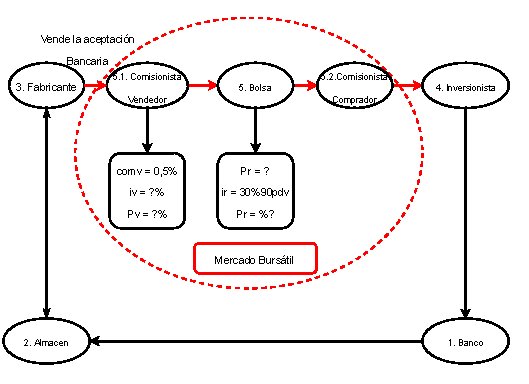
\includegraphics[trim=-78 -5 -78 -5]{3_Capitulo/img/ejemplos/7/Capitulo3Ejercicio7a3.pdf} }  \\ \hline
  %%%%%% FIN FLUJO DE CAJA

%%%%% INICIO DECLARACIÓN FORMULAS
  \rowcolor[HTML]{FFB183}
  \multicolumn{2}{|c|}{\cellcolor[HTML]{FFB183}\textbf{4. Declaración de formulas}}                  \\ \hline
  \multicolumn{2}{|C{\textwidth}|}{
  $F = P(1 + i)^n $ \hspace{2mm} Valor futuro 
  
  $I_r$ para calcular $p_r$    

  $i_r$ comv para calcular $p_c$

  $V_v=?$
  }
  \\ \hline
  %%%%% FIn  DECLARACIÓN FORMULAS
  \rowcolor[HTML]{FFB183}
  \multicolumn{2}{|c|}{\cellcolor[HTML]{FFB183}\textbf{5. Desarrollo matemático}}                    \\ \hline
  %Mezclamos 3 columnas y pondremos el dibujo
  %%%%%%%%%%%%% INSERCIÓN DE LA IMAGEN
  %Deberán descargar las imágenes respectivas del drive y pegarlas en la carpeta
  %n_capitulo/img/ejemplos/1/capitulo1ejemplo1.pdf  (el /1/ es el numero del ejemplo)
  \multicolumn{2}{|C{\linewidth}|}{

  $P_r =   100 \ COP (1 + 0,30)^\frac{-90}{365} = 93,7356\% \equiv 4{.}686{.}780 \ COP$

  $i_v = 0,5\% \hspace{1mm} pdv + 30\%\hspace{1mm}pdv = 30,5\% \hspace{1mm}pdv$

  $Pv =  100\ COP(1 + 0, 3050)^\frac{-90}{365}= 93,6469\% \equiv  4{.}682{.}345\ COP $

  }                                                                                                  \\ \hline

  %%%%% INICIO DECLARACIÓN FORMULAS
  %%%%%%%%%%% INICIO TITULO
  \rowcolor[HTML]{FFB183}

  %%%%%% INICIO RESPUESTA
  \rowcolor[HTML]{FFB183}
  %%%%%%%%%%INICIO TITULO
  \multicolumn{2}{|c|}{\cellcolor[HTML]{FFB183}\textbf{6. Respuesta}}                                \\ \hline
  %%%%%%%%%% FIN TITULO
  %%%%%%%%%% INICIO RESPUESTA MATEMÁTICA
  \multicolumn{2}{|C{\textwidth}|}{
  $Pr =   4{.}686{.}780 \ COP$

  $iv = 30, 5\% \hspace{1mm} pdv$

  $Pv =   4{.}682{.}345 \ COP$

  $P_v = 93,6469\% < p_r = 93,7356?\%$
  }                                                                                                  \\ \hline
  %%%%%%%%%% FIN MATEMÁTICAS

  
  %%%%%% FIN RESPUESTA
 \end{longtable}
 %Se crean dos lineas en blanco para que no quede el siguiente texto tan pegado
 %\newline \newline %USARLO SI CREES QUE ES NECESARIO
\end{center}


b) Para 40 días antes del vencimiento:
%La tabla ira centrada
\begin{center}
 \renewcommand{\arraystretch}{1.5}% Margenes de las celdas
 %Creación de la cuadricula de 3 columnas
 \begin{longtable}[H]{|p{0.5\linewidth}|p{0.5\linewidth}|}
  %Creamos una linea horizontal
  \hline
  %Definimos el color de la primera fila
  \rowcolor[HTML]{FFB183}
  %%%%% INICIO ASIGNACIÓN FECHA FOCAL %%%%%%%
  %%%%%%%%%% INICIO TITULO
  %Lo que se hace aquí es mezclar las 3 columnas en una sola
  \multicolumn{2}{|c|}{\cellcolor[HTML]{FFB183}\textbf{1. Asignación período focal}}                   \\ \hline
  %%%%%%%%%% FIN TITULO
  %%%%% INICIO DECLARACIÓN DE VARIABLES %%%%%%%
  \multicolumn{2}{|c|}{$pf = 40 \textit{ pdv}$}                                                      \\ \hline
  %%%%%%%%%% INICIO TITULO
  %Lo que se hace aquí es mezclar las 3 columnas en una sola
  \multicolumn{2}{|c|}{\cellcolor[HTML]{FFB183}\textbf{2. Declaración de variables}}                 \\ \hline
  %%%%%%%%%% FIN TITULO
  %%%%%%%%%% INICIO DE MATEMÁTICAS
  %Cada & hace referencia al paso de la siguiente columna
  $F =  100 \ COP$                   & $P_r = ? \ COP$                                                            \\
  $n  = \frac{40}{365} = 0.110\% \ pdv$     & $P_v=?\ COP$                                                             \\
  $i_r = 30\%\textit{ pdv}  $  & $i_v=?\% $                                                             \\
  $com_v = 0,5\%\textit{ pdv}$ &    $i_{r}+comv = P_{v}$                                                                 \\ \hline
  %%%%%%%%%% FIN DE MATEMÁTICAS
  %%%%% FIN DECLARACIÓN DE VARIABLES


  %%%%% INICIO FLUJO DE CAJA
  \rowcolor[HTML]{FFB183}
  \multicolumn{2}{|c|}{\cellcolor[HTML]{FFB183}\textbf{3. Diagrama de flujo de caja}}                \\ \hline
\multicolumn{2}{|c|}{ \includegraphics[trim=-78 -5 -78 -5]{3_Capitulo/img/ejemplos/7/capitulo3ejercicio7a3.pdf} }  \\ \hline
  %%%%%% FIN FLUJO DE CAJA

%%%%% INICIO DECLARACIÓN FORMULAS
  \rowcolor[HTML]{FFB183}
  \multicolumn{2}{|c|}{\cellcolor[HTML]{FFB183}\textbf{4. Declaración de formulas}}                  \\ \hline
  \multicolumn{2}{|C{\textwidth}|}{
  $F = P(1 + i)^n $ \hspace{2mm} Valor futuro 
  
  $I_r$ para calcular $p_r$    

  $i_r$ comv para calcular $p_c$

  $V_v=?$
  }
  \\ \hline
  %%%%% FIn  DECLARACIÓN FORMULAS
  \rowcolor[HTML]{FFB183}
  \multicolumn{2}{|c|}{\cellcolor[HTML]{FFB183}\textbf{5. Desarrollo matemático}}                    \\ \hline
  %Mezclamos 3 columnas y pondremos el dibujo
  %%%%%%%%%%%%% INSERCIÓN DE LA IMAGEN
  %Deberán descargar las imágenes respectivas del drive y pegarlas en la carpeta
  %n_capitulo/img/ejemplos/1/capitulo1ejemplo1.pdf  (el /1/ es el numero del ejemplo)
  \multicolumn{2}{|C{\linewidth}|}{

  $P_r =   100 \ COP (1 + 0,30)^\frac{-40}{365} = 97,165\% \equiv 4{.}858{.}285 \ COP$

  $i_v = 0,5\% \hspace{1mm} pdv + 30\%\hspace{1mm}pdv = 30,5\% \hspace{1mm}pdv$

  $Pv =  100\ COP(1 + 0, 3050)^\frac{-40}{365}= 97,1248\% \equiv  4{.}856{.}240\ COP $

  }                                                                                                  \\ \hline

  %%%%% INICIO DECLARACIÓN FORMULAS
  %%%%%%%%%%% INICIO TITULO
  \rowcolor[HTML]{FFB183}

  %%%%%% INICIO RESPUESTA
  \rowcolor[HTML]{FFB183}
  %%%%%%%%%%INICIO TITULO
  \multicolumn{2}{|c|}{\cellcolor[HTML]{FFB183}\textbf{6. Respuesta}}                                \\ \hline
  %%%%%%%%%% FIN TITULO
  %%%%%%%%%% INICIO RESPUESTA MATEMÁTICA
  \multicolumn{2}{|C{\textwidth}|}{
  $Pr =  4{.}858{.}285 \ COP$

  $iv = 30, 5\% \hspace{1mm} pdv$

  $Pv = 4{.}856{.}240 \ COP$

  $P_v = 97,1248\% < p_r = 97,165\%$
  }                                                                                                  \\ \hline
  %%%%%%%%%% FIN MATEMÁTICAS

  
  %%%%%% FIN RESPUESTA
 \end{longtable}
 %Se crean dos lineas en blanco para que no quede el siguiente texto tan pegado
 %\newline \newline %USARLO SI CREES QUE ES NECESARIO
\end{center}


c) Para 10 días antes del vencimiento:

%La tabla ira centrada
\begin{center}
 \renewcommand{\arraystretch}{1.5}% Margenes de las celdas
 %Creación de la cuadricula de 3 columnas
 \begin{longtable}[H]{|p{0.5\linewidth}|p{0.5\linewidth}|}
  %Creamos una linea horizontal
  \hline
  %Definimos el color de la primera fila
  \rowcolor[HTML]{FFB183}
  %%%%% INICIO ASIGNACIÓN FECHA FOCAL %%%%%%%
  %%%%%%%%%% INICIO TITULO
  %Lo que se hace aquí es mezclar las 3 columnas en una sola
  \multicolumn{2}{|c|}{\cellcolor[HTML]{FFB183}\textbf{1. Asignación período focal}}                   \\ \hline
  %%%%%%%%%% FIN TITULO
  %%%%% INICIO DECLARACIÓN DE VARIABLES %%%%%%%
  \multicolumn{2}{|c|}{$pf = 10 \textit{ pdv}$}                                                      \\ \hline
  %%%%%%%%%% INICIO TITULO
  %Lo que se hace aquí es mezclar las 3 columnas en una sola
  \multicolumn{2}{|c|}{\cellcolor[HTML]{FFB183}\textbf{2. Declaración de variables}}                 \\ \hline
  %%%%%%%%%% FIN TITULO
  %%%%%%%%%% INICIO DE MATEMÁTICAS
  %Cada & hace referencia al paso de la siguiente columna
  $F =  100 \ COP$                   & $P_r = ? \ COP$                                                            \\
  $n  = \frac{10}{365} = 0.247\% \ pdv$     & $P_v=?\ COP$                                                             \\
  $i_r = 30\%\textit{ pdv}  $  & $i_v=?\% $                                                             \\
  $com_v = 0,5\%\textit{ pdv}$ &    $i_{r}+comv = P_{v}$                                                                 \\ \hline
  %%%%%%%%%% FIN DE MATEMÁTICAS
  %%%%% FIN DECLARACIÓN DE VARIABLES


  %%%%% INICIO FLUJO DE CAJA
  \rowcolor[HTML]{FFB183}
  \multicolumn{2}{|c|}{\cellcolor[HTML]{FFB183}\textbf{3. Diagrama de flujo de caja}}                \\ \hline
 \multicolumn{2}{|c|}{ \includegraphics[trim=-78 -5 -78 -5]{3_Capitulo/img/ejemplos/7/capitulo3ejercicio7a3.pdf} }  \\ \hline
  %%%%%% FIN FLUJO DE CAJA

%%%%% INICIO DECLARACIÓN FORMULAS
  \rowcolor[HTML]{FFB183}
  \multicolumn{2}{|c|}{\cellcolor[HTML]{FFB183}\textbf{4. Declaración de formulas}}                  \\ \hline
  \multicolumn{2}{|C{\textwidth}|}{
  $F = P(1 + i)^n $ \hspace{2mm} Valor futuro 
  
  $I_r$ para calcular $p_r$    

  $i_r$ comv para calcular $p_c$

  $V_v=?$
  }
  \\ \hline
  %%%%% FIn  DECLARACIÓN FORMULAS
  \rowcolor[HTML]{FFB183}
  \multicolumn{2}{|c|}{\cellcolor[HTML]{FFB183}\textbf{5. Desarrollo matemático}}                    \\ \hline
  %Mezclamos 3 columnas y pondremos el dibujo
  %%%%%%%%%%%%% INSERCIÓN DE LA IMAGEN
  %Deberán descargar las imágenes respectivas del drive y pegarlas en la carpeta
  %n_capitulo/img/ejemplos/1/capitulo1ejemplo1.pdf  (el /1/ es el numero del ejemplo)
  \multicolumn{2}{|C{\linewidth}|}{

  $P_r =   100 \ COP (1 + 0,30)^\frac{-10}{365} = 99,2838\% \equiv 4{.}964{.}190 \ COP$

  $i_v = 0,5\% \hspace{1mm} pdv + 30\%\hspace{1mm}pdv = 30,5\% \hspace{1mm}pdv$

  $Pv =  100\ COP(1 + 0, 3050)^\frac{-10}{365}= 99,2733\% \equiv  4{.}963{.}665\ COP $

  }                                                                                                  \\ \hline

  %%%%% INICIO DECLARACIÓN FORMULAS
  %%%%%%%%%%% INICIO TITULO
  \rowcolor[HTML]{FFB183}

  %%%%%% INICIO RESPUESTA
  \rowcolor[HTML]{FFB183}
  %%%%%%%%%%INICIO TITULO
  \multicolumn{2}{|c|}{\cellcolor[HTML]{FFB183}\textbf{6. Respuesta}}                                \\ \hline
  %%%%%%%%%% FIN TITULO
  %%%%%%%%%% INICIO RESPUESTA MATEMÁTICA
  \multicolumn{2}{|C{\textwidth}|}{
  \newline
  $Pr =  4{.}964{.}190\ COP$

  $iv = 30, 5\% \hspace{1mm} pdv$

  $Pv =  4{.}963{.}665 \ COP$

  $P_v = 97,1248\% < p_r = 97,165\%$
  \newline
  }                                                                                                  \\ \hline
  %%%%%%%%%% FIN MATEMÁTICAS

  
  %%%%%% FIN RESPUESTA
 \end{longtable}
 %Se crean dos lineas en blanco para que no quede el siguiente texto tan pegado
 %\newline \newline %USARLO SI CREES QUE ES NECESARIO

\end{center}\

\begin{center}
 \textbf{Tabla resumen para el vendedor}
\end{center}

\begin{center}
\renewcommand{\arraystretch}{1.5} % Ajusta la altura de la tabla
\setlength{\tabcolsep}{1pt} % Ajusta el espaciado de las columnas
\begin{tabular}{|c|c|c|c|c|c|c|}
\hline
\multirow{2}{*}{} & \multicolumn{3}{|c|}{\textbf{Mercado no bursátil}}  & \multicolumn{3}{|c|}{\textbf{Mercado bursátil}} \\
\cline{2-7}
& \textbf{90 DÍAS} & \textbf{40 DÍAS} & \textbf{10 DÍAS} & \textbf{90 DÍAS} & \textbf{40 DÍAS} & \textbf{10 DÍAS} \\
\cline{1-7}
\textbf{Tasa} & 30\% pdv & 30\% pdv & 30\% pdv & 30,5\% pdv & 30,5\% pdv & 30,5\% pdv \\
\hline
\textbf{Precio} & 93,73\% COP & 97,16\% COP & 99,28\% COP & 93,64\% COP & 97,12\% COP & 99,27\% COP \\
\hline
\textbf{Valor} & 4.650.000COP & 4.850.000COP & 4.950.000COP & 4.682.345COP & 4.856.240COP & 4.963.665COP \\
\hline
\textbf{Comisión} & 0\% pdv & 0\% pdv & 0\% pdv & 0,5\% pdv & 0,5\% pdv & 0,5\% pdv \\
\hline
\end{tabular}
\end{center}

%%%%%%%%%%%%%%%%%%%%%%%%%%EJERCICIO 8 %%%%%%%%%%%%%%%%%%%%%%%%%%%
\newpage
\textbf{Ejemplo 8}\\
Supongamos que un inversionista desea adquirir la aceptación bancaria del ejemplo anterior, la cual figura con una tasa de registro del 30\% periódico 40 días vencido y con precio de registro $P_r =  97,65 COP$ pero él también sabe que para adquirirla deberá pagar una comisión a un corredor de bolsa lo cual hará variar el precio que él debe pagar y también la rentabilidad que él pueda obtener. Supongamos que la comisión que cobra un corredor por la compra es del 0,475\% periodo 40 días periodo vencido ¿Cuál es el precio del inversionista Pc =  ? COP , que incluye la comisión del comisionista vendedor, el precio de registro y la comisión de bolsa del comprador. El punto de referencia es el precio de registro $P_r$ ¿Cuál es la rentabilidad del inversionista $i_c =? \%?$ periódica 40 días vencido, o $j=? \hspace{0.5mm} nadv$
%\newpage %USAR SOLO SI EL SOLUCIÓN QUEDA SOLO Y ES NECESARIO BAJARLO A LA SIGUIENTE PAGINA

\textbf{Solución.}
%La tabla ira centrada
\begin{center}
 \renewcommand{\arraystretch}{1.5}% Margenes de las celdas
 %Creación de la cuadricula de 3 columnas
 \begin{longtable}[H]{|p{0.5\linewidth}|p{0.5\linewidth}|}
  %Creamos una linea horizontal
  \hline
  %Definimos el color de la primera fila
  \rowcolor[HTML]{FFB183}
  %%%%% INICIO ASIGNACIÓN FECHA FOCAL %%%%%%%
  %%%%%%%%%% INICIO TITULO
  %Lo que se hace aquí es mezclar las 3 columnas en una sola
  \multicolumn{2}{|c|}{\cellcolor[HTML]{FFB183}\textbf{1. Asignación período focal}}                  \\ \hline
  %%%%%%%%%% FIN TITULO
  %%%%% INICIO DECLARACIÓN DE VARIABLES %%%%%%%
  \multicolumn{2}{|c|}{$pf = 40 \textit{ pdv}$}                                                     \\ \hline
  %%%%%%%%%% INICIO TITULO
  %Lo que se hace aquí es mezclar las 3 columnas en una sola
  \multicolumn{2}{|c|}{\cellcolor[HTML]{FFB183}\textbf{2. Declaración de variables}}                \\ \hline
  %%%%%%%%%% FIN TITULO
  %%%%%%%%%% INICIO DE MATEMÁTICAS
  %Cada & hace referencia al paso de la siguiente columna
  $i_c = 30\% -0,475\% = 29,525\% \hspace{1mm} p40dv$ & $P_R=?$                                     \\
  $P_c =  ? COP$                                         &                                             \\
  $n= \frac{40}{365} \hspace{1mm} p(40das) $          &                                             \\ \hline
  %%%%%%%%%% FIN DE MATEMÁTICAS
  %%%%% FIN DECLARACIÓN DE VARIABLES

  \rowcolor[HTML]{FFB183}
  \multicolumn{2}{|c|}{\cellcolor[HTML]{FFB183}\textbf{3. Diagrama de flujo de caja}}               \\ \hline
  \multicolumn{2}{|c|}{ 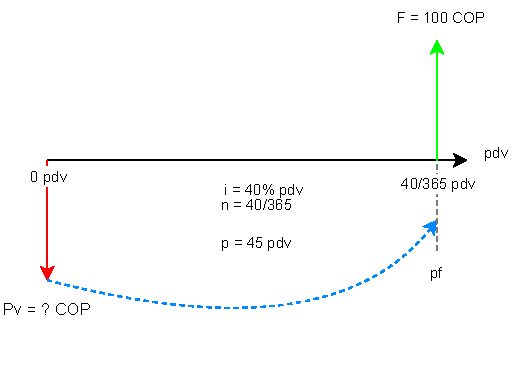
\includegraphics[trim=-78 0 -78 0]{3_Capitulo/img/ejemplos/8/capitulo3ejercicio8.pdf} }  \\ \hline
  %%%%% INICIO FLUJO DE CAJA
  \rowcolor[HTML]{FFB183}
  \multicolumn{2}{|c|}{\cellcolor[HTML]{FFB183}\textbf{4. DECLARACIÓN de formulas}}                 \\ \hline
  %Mezclamos 3 columnas y pondremos el dibujo
  %%%%%%%%%%%%% INSERCIÓN DE LA IMAGEN
  %Deberán descargar las imágenes respectivas del drive y pegarlas en la carpeta
  %n_capitulo/img/ejemplos/1/capitulo1ejemplo1.pdf  (el /1/ es el numero del ejemplo)
  \multicolumn{2}{|c|}{ $P = F(1 + i)^n $ Valor presente }                                          \\ \hline
  %%%%%%%%%%%%% FIN INSERCIÓN DE IMAGEN
  %%%%%FIN FLUJO DE CAJA


  %%%%%% INICIO DESARROLLO MATEMÁTICO
  \rowcolor[HTML]{FFB183}
  %%%%%%%%%%INICIO TITULO
  \multicolumn{2}{|c|}{\cellcolor[HTML]{FFB183}\textbf{5. Desarrollo matemático}}                   \\ \hline
  %%%%%%%%%% FIN TITULO
  %%%%%%%%%% INICIO MATEMÁTICAS
  \multicolumn{2}{|C{\linewidth}|}{
  $P_c =  100 COP(1 + 0,29525)\frac{40}{365} = 97,204 COP$ Ecuación de valor

  $P_R = 0,972047( 5{.}000{.}000 COP) =  4{.}860{.}245 COP$

  $P_c - P_R =  4{.}860{.}235 COP -  4{.}858{.}285 COP = 1{.}950 COP$
  }                                                                                                 \\ \hline

  %%%%%%%%%% FIN MATEMÁTICAS
  %%%%%% FIN DESARROLLO MATEMÁTICO
  %%%%%% INICIO RESPUESTA
  \rowcolor[HTML]{FFB183}
  %%%%%%%%%%INICIO TITULO
  \multicolumn{2}{|c|}{\cellcolor[HTML]{FFB183}\textbf{6. Respuesta}}                               \\ \hline
  %%%%%%%%%% FIN TITULO
  %%%%%%%%%% INICIO RESPUESTA MATEMÁTICA
  \multicolumn{2}{|C{\textwidth}|}{
  $P_R =  4{.}860{.}245 COP$
  }                                                                                                 \\ \hline


  %%%%%%%%%% FIN MATEMÁTICAS
  %%%%%% FIN RESPUESTA
 \end{longtable}
 %Se crean dos lineas en blanco para que no quede el siguiente texto tan pegado
 %\newline \newline %USARLO SI CREES QUE ES NECESARIO
\end{center}
%%%%%%%%%%%%%%%%%%%%%%%%%%FIN EJERCICIO 8 %%%%%%%%%%%%%%%%%%%%%%%%%%%

\newpage
\textbf{Ejemplo 9}\\
El dueño del almacén solicita al banco una aceptación bancaria por 5 millones COP, que
entregará al fabricante o proveedor para que le entreguen la mercancía. El banco presta
este servicio y le cobra al almacén una comisión del 1\% mensual trimestre anticipado sobre
el valor de la aceptación. Considerar el iva del 16\% del valor monetario de la comisión
bancaria.\\
a) Comisión bancaria que debe pagar el almacén por su expedición.\\
Si el fabricante vende la aceptación faltando 40 días a una tasa del 30\% pdv y por ello el
precio de registro en bolsa es de $P_{R}$ = 4.850.000 COP, y la bolsa le hace una retención en la fuente sobre los rendimientos del 7\% calcular: \\
b) El precio de compra Pc incluyendo la retención en la fuente y excluyendo la comisión
del comisionista comprador. \\ 
\textbf{Solución.}
%La tabla ira centrada
\begin{center}
	\renewcommand{\arraystretch}{1.5}% Margenes de las celdas
	%Creación de la cuadricula de 3 columnas
\begin{longtable}[H]{|c|c|c|}
		%Creamos una linea horizontal
\hline
		%Definimos el color de la primera fila
\rowcolor[HTML]{FFB183}
		%%%%% INICIO ASIGNACIÓN PERIODO FOCAL %%%%%%%
		%%%%%%%%%% INICIO TITULO
		%Lo que se hace aquí es mezclar las 3 columnas en una sola
\multicolumn{3}{|c|}{\cellcolor[HTML]{FFB183}\textbf{1. Asignación período focal}}   \\ \hline
\multicolumn{3}{|c|} {$pf = 40 pdv$} \\ \hline
		%%%%%%%%%% FIN TITULO
  %%%%% INICIO DECLARACIÓN FORMULAS
  
%%%%%%%%%%% INICIO TITULO
\rowcolor[HTML]{FFB183}
\multicolumn{3}{|c|}{\cellcolor[HTML]{FFB183}\textbf{2. Declaración de variables}}    \\ \hline
%%%%%%%%%%% FIN TITULO
%%%%%%%%%%% INICIO MATEMÁTICAS
\begin{minipage}{9cm}
\textit{Com bancaria = 1\% mensual trimestre anticipado del valor de la aceptación }   \end{minipage}      &  \multicolumn{2}{c|}{$ V_{com} = \textit{? COP Valor comisión bancaria} $}
\\ 
\begin{minipage}{9cm}
\textit{iva = 16\% de la com bancaria\\
$n = \frac{40}{365} p(40 dv)$\\
P\textsubscript{R} = 4.858.285 COP\\
R\textsubscript{F} = 7\% sobre las utilidades (F - P\textsubscript{R})\\}   \end{minipage}      & \multicolumn{2}{c|}{$ P_{c} = \textit{? COP} $}
\\ \hline
%%%%%%%%%% FIN MATEMÁTICAS
		%%%%% INICIO FLUJO DE CAJA
\rowcolor[HTML]{FFB183}
\multicolumn{3}{|c|}{\cellcolor[HTML]{FFB183}\textbf{3. Diagrama de flujo de caja}} \\ \hline
		%Mezclamos 3 columnas y pondremos el dibujo
		%%%%%%%%%%%%% INSERCIÓN DE LA IMAGEN
		%Deberán descargar las imágenes respectivas del drive y pegarlas en la carpeta
		%n_capitulo/img/ejemplos/1/capitulo1ejemplo1.pdf  (el /1/ es el numero del ejemplo)
\multicolumn{3}{|p{\textwidth}|}{No aplica porque el enunciado ya entrega el precio de registro y el objetivo del ejercicio es
aplicar los conceptos de expedición, aceptaciones bancarias, valor del iva y de retención
en la fuente.}  \\ \hline
		%%%%%%%%%%%%% FIN INSERCIÓN DE IMAGEN
		%%%%%FIN FLUJO DE CAJA
		
		
		
		%%%%% INICIO DECLARACIÓN FORMULAS
		%%%%%%%%%%% INICIO TITULO
\rowcolor[HTML]{FFB183}
\multicolumn{3}{|c|}{\cellcolor[HTML]{FFB183}\textbf{4. Declaración de fórmulas}}    \\ \hline
		%%%%%%%%%%% FIN TITULO
		%%%%%%%%%%% INICIO MATEMÁTICAS
\multicolumn{3}{|c|}{\textit{a) Com bancaria = F(\% que cobre el banco + iva)}} \\
\multicolumn{3}{|c|}{\textit{iva = 16\% $\cdot$ Com bancaria}} \\
\multicolumn{3}{|c|}{\textit{b) $P_{c} = P_{R} + R_{F}$}} \\
\multicolumn{3}{|c|}{\textit{$R_{F} = 7\%(F-P_{R})$}} \\
\hline	
	
		%%%%%%%%%% FIN MATEMÁTICAS
		%%%%%% INICIO DESARROLLO MATEMÁTICO
\rowcolor[HTML]{FFB183}
		%%%%%%%%%%INICIO TITULO
\multicolumn{3}{|c|}{\cellcolor[HTML]{FFB183}\textbf{5. Desarrollo matemático}}       \\ \hline
		%%%%%%%%%% FIN TITULO
		%%%%%%%%%% INICIO MATEMÁTICAS

\multicolumn{3}{|p{\textwidth}|}{\textit{a) Com bancaria = 5.000.000 $COP\cdot 0,01$ (3 meses) = 150.000 COP} }
\\
\multicolumn{3}{|p{\textwidth}|}{\textit{iva = 150.000 COP(0,16) = 24.000 COP} } \\
\multicolumn{3}{|p{\textwidth}|}{\textit{Com bancaria + iva = 150.00 COP + 24.000 COP = 174.000 COP que afecta al almacén} } \\
\multicolumn{3}{|p{\textwidth}|}{\textit{b) $R_{F}$ = 0,07 (5.000.000 COP - 4.858.285 COP) = 9.920 COP} }
\\ \hline
		
\hline
		
		%%%%%%%%%% FIN MATEMÁTICAS
		%%%%%% FIN DESARROLLO MATEMÁTICO
		%%%%%% INICIO RESPUESTA
\rowcolor[HTML]{FFB183}
		%%%%%%%%%%INICIO TITULO
\multicolumn{3}{|c|}{\cellcolor[HTML]{FFB183}\textbf{6. Respuesta}}   \\ \hline
		%%%%%%%%%% FIN TITULO
		%%%%%%%%%% INICIO RESPUESTA MATEMÁTICA
\multicolumn{3}{|c|}{a) Com bancaria = 174.000 COP} \\
\multicolumn{3}{|c|}{B) $P_{c}$ = 4.858.285 COP + 9.920 COP  = 4.868.205 COP} 
\\ \hline
		
		
		%%%%%%%%%% FIN MATEMÁTICAS
		%%%%%% FIN RESPUESTA
	\end{longtable}
	%Se crean dos lineas en blanco para que no quede el siguiente texto tan pegado
	%\newline \newline %USARLO SI CREES QUE ES NECESARIO
\end{center}
%%%%%%%%%%%%%%%%%%%%%%%%%%FIN 

\newpage
	\textbf{Ejemplo 10}\newline
Supongamos que faltando 10 días para el vencimiento el inversionista del ejemplo anterior decide venderlo y para esta época se están negociando en Bolsa con una tasa del 28\% período 10 días vencido, por lo tanto la tasa de registro debe ser del 28\% período 10 días Vencido. El valor de compra del ejemplo anterior es de 97,204\% COP (faltando 40 días) Suponer el año de 365 días. Calcular:\\
1. El precio de registro en bolsa. \\
2. La retención en la fuente que debe reconocer al vendedor. \\
3. La tasa del vendedor. \\
4. El precio de vendedor. \\
5. Valor de venta.  \\
6. Tasa del comprador. \\
7. Valor del comprador. \newline
\textbf{Solución.
\newline}
\begin{center}
    \renewcommand{\arraystretch}{1.5}% Margenes de las celdas
    %Creación de la cuadricula
    \begin{longtable}[H]{|c|c|c| }
        %Creamos una linea horizontal
        \hline
        %Definimos el color de la primera fila
        \rowcolor[HTML]{FFB183}
        %%%%% INICIO ASIGNACIÓN FECHA FOCAL %%%%%%%
        %%%%%%%%%% INICIO TITULO
        %Lo que se hace aquí es mezclar las 3 columnas en una sola
        \multicolumn{3}{|c|}{\cellcolor[HTML]{FFB183}\textbf{1. Asignación período focal}}   \\ \hline
        %%%%%%%%%% FIN TITULO
        %%%%% INICIO DECLARACIÓN DE VARIABLES %%%%%%%
        \multicolumn{3}{|c|}{$pf = 10 pdv $} \\ \hline
        %Definimos el color de la primera fila
        \rowcolor[HTML]{FFB183}
        %%%%% INICIO DECLARACIÓN DE VARIABLES %%%%%%%
        %%%%%%%%%% INICIO TITULO
        \multicolumn{3}{|c|}{\cellcolor[HTML]{FFB183}\textbf{2. Declaración de variables}}                                                                                   \\ \hline
        %%%%%%%%%% FIN TITULO
        %%%%%%%%%% INICIO DE MATEMÁTICAS
        $F =  100 COP  $ & 
        \multicolumn{2}{c|}{$ a) P_{r} =  ? COP;$\hspace{0.5cm}$ b) i_{v} =  ? \% pdv $} \\
        $ n = 10/365 = 0,027 pdv $ &
        \multicolumn{2}{c|}{$ c) P_{v} = ? COP;$\hspace{0.5cm}$ d) V_{v} =  ? COP $} \\
        $ n = (40-10)/365 pdv $ &
        \multicolumn{2}{c|}{ $ e) i_{c} = ? \% pdv;$\hspace{0.5cm}$ f) P_{c} = ? COP $ } \\
        $ i_{r} = 28\% 10 pdv $     & 
        \multicolumn{2}{c|}{ $ g) V_{c} = ? COP;$\hspace{0.5cm}$ h) R_{F} = ? COP $ } \\
        $ P_{c1} =  97,204 COP $   & 
        \multicolumn{2}{c|}{ $  $ }
        \\ \hline
        %%%%%%%%%% FIN DE MATEMÁTICAS
        %%%%% FIN DECLARACIÓN DE VARIABLES
        
        
        %%%%% INICIO FLUJO DE CAJA
        \rowcolor[HTML]{FFB183}
        \multicolumn{3}{|c|}{\cellcolor[HTML]{FFB183}\textbf{3. Diagrama de flujo de caja}}                                                                                  \\ \hline
        %Mezclamos 3 columnas y pondremos el dibujo
        %%%%%%%%%%%%% INSERCIÓN DE LA IMAGEN
\multicolumn{2}{|c|}{ 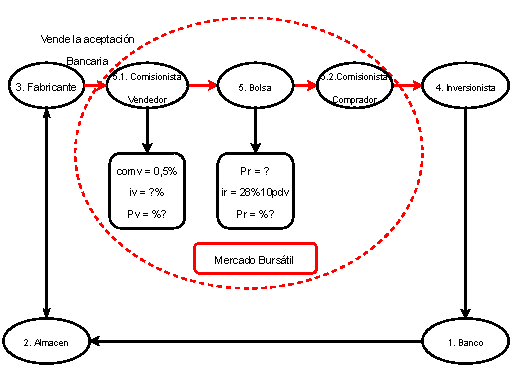
\includegraphics[trim=-90 -5 -90 -5]{3_Capitulo/img/ejemplos/10/capitulo3ejercicio10.pdf} }                                                                                      \\ \hline
        %%%%%%%%%%%%% FIN INSERCIÓN DE IMAGEN
        %%%%%FIN FLUJO DE CAJA
        
        
        
        %%%%% INICIO DECLARACIÓN FORMULAS
        %%%%%%%%%%% INICIO TITULO
        \rowcolor[HTML]{FFB183}
        \multicolumn{3}{|c|}{\cellcolor[HTML]{FFB183}\textbf{4. Declaración de fórmulas}}                                                                                    \\ \hline
        %%%%%%%%%%% FIN TITULO
        %%%%%%%%%%% INICIO MATEMÁTICAS
    
         \multicolumn{3}{|c|}{$P=F(1+i)^{-n}$\hspace{35pt}\textit{Valor presente}
         \hspace{0.3cm}}\\
         \multicolumn{3}{|c|}{$R_{F} = (F - P)*0,7$\hspace{35pt}\textit{Retención en la fuente}
         \hspace{0.3cm}}\\
         \multicolumn{3}{|c|}{$V_{V} = P_{V} * V_{total}$\hspace{35pt}\textit{}
         \hspace{0.3cm}}\\
         \multicolumn{3}{|c|}{$V_{C} = P_{C} * V_{total}$\hspace{35pt}\textit{}
         \hspace{0.3cm}}\\
        
         
         \hline
        %%%%%%%%%% FIN MATEMÁTICAS
        %%%%%% INICIO DESARROLLO MATEMÁTICO
        \rowcolor[HTML]{FFB183}
        %%%%%%%%%%INICIO TITULO
        \multicolumn{3}{|c|}{\cellcolor[HTML]{FFB183}\textbf{5. Desarrollo matemático}}                                                                                      \\ \hline
        %%%%%%%%%% FIN TITULO
        %%%%%%%%%% INICIO MATEMÁTICAS
         \multicolumn{3}{|c|}{$ a) P_{r} = 100 COP * (1 + 0,28)^{-10/365} = 99,3260\% COP$
         \hspace{0.3cm}}\\
         \multicolumn{3}{|c|}{$ b) 97,204 COP = 99.3260 (1+i)^{-30/365} => i_{v} = 6,4\% pdv$
         \hspace{0.3cm}}\\
         \multicolumn{3}{|c|}{$ d) V_{v} = 0,972 COP * 5{.}000{.}000 COP = 4{.}860{.}000 COP $
         \hspace{0.3cm}}\\
         \multicolumn{3}{|c|}{$ e) 99,3260 \% = 100 COP (1+ i)^{-10/365} => i = 9,84\%$
         \hspace{0.3cm}}\\
         \multicolumn{3}{|c|}{$ f) P_{c} = 100 COP (1 + 0,0984)^{-10/365} = 90,16\% COP $
         \hspace{0.3cm}}\\
         \multicolumn{3}{|c|}{$ g) V_{c} = 0,9016 * 5{.}000{.}000 COP = 4{.}508{.}000 COP $
         \hspace{0.3cm}}\\
         \multicolumn{3}{|c|}{$ h) R_{F} = 0,07(5{.}000{.}000 - 97,204) $
         \hspace{0.3cm}}\\
         
        %%%%%%%%%% FIN MATEMÁTICAS
        %%%%%% FIN DESARROLLO MATEMÁTICO
        
        \rowcolor[HTML]{FFB183}
        \multicolumn{3}{|c|}{\cellcolor[HTML]{FFB183}\textbf{6. Respuesta}} \\ \hline    
        
        \multicolumn{3}{|c|}{$P_{r} = 4{.}964{.}190 COP $} \\ \hline
    \end{longtable}
    %Se crean dos lineas en blanco para que no quede el siguiente texto tan pegado
\end{center}


\textbf{Ejemplo 11}\newline
	Una aceptación bancaria por 80 millones COP con fecha de vencimiento el 17 de diciembre de 1999 es adquirida en 22 de julio de 1999 por un primer inversionista con una tasa del de 28\% período 28 días vencidos y es cedida a un segundo inversionista el 14 de octubre de 1999. Si el segundo inversionista desea ganarse el 32\% período días vencido utilice un año de 360 (año de 360 días) \\
	¿Cuál es la ganancia en pesos del primer inversionista? \\
	¿Cuál es la rentabilidad periódica días vencido del primer inversionista?\\

	\textbf{Solución.}
	\begin{center}

		\renewcommand{\arraystretch}{1.5}% Margenes de las celdas
		%Creación de la cuadricula
		\begin{longtable}[H]{|c|c|c| }
			%Creamos una linea horizontal
			\hline
			%Definimos el color de la primera fila
			\rowcolor[HTML]{FFB183}
			%%%%% INICIO ASIGNACIÓN FECHA FOCAL %%%%%%%
			%%%%%%%%%% INICIO TITULO
			%Lo que se hace aquí es mezclar las 3 columnas en una sola
			\multicolumn{3}{|c|}{\cellcolor[HTML]{FFB183}\textbf{1. Asignación período focal}}   \\ \hline
			%%%%%%%%%% FIN TITULO
			%%%%% INICIO DECLARACIÓN DE VARIABLES %%%%%%%
			\multicolumn{3}{|c|}{$pf = 0 pdv$} \\ \hline
			%Definimos el color de la primera fila
			\rowcolor[HTML]{FFB183}
			%%%%% INICIO DECLARACIÓN DE VARIABLES %%%%%%%
			%%%%%%%%%% INICIO TITULO
			\multicolumn{3}{|c|}{\cellcolor[HTML]{FFB183}\textbf{2. Declaración de variables}}                                                                                   \\ \hline
			%%%%%%%%%% FIN TITULO
			%%%%%%%%%% INICIO DE MATEMÁTICAS
			$i_{1} = 28 \% pdv$                                     & \multicolumn{2}{c|}{$ n_{1} = (145/365) pdv $} \\
			$i_{2} = 32\% pdv \hspace{0.3cm} $	& \multicolumn{2}{c|}{$ n_{2} = (63/365) pdv $} \\
			$P_{C2} - P_{C1} = ? $ & \multicolumn{2}{c|}{$ n_{3} = 0 pdv $}\\ \hline
			%%%%%%%%%% FIN DE MATEMÁTICAS
			%%%%% FIN DECLARACIÓN DE VARIABLES
			
			
			%%%%% INICIO FLUJO DE CAJA
			\rowcolor[HTML]{FFB183}
			\multicolumn{3}{|c|}{\cellcolor[HTML]{FFB183}\textbf{3. Diagrama de flujo de caja}}                                                                                  \\ \hline
			%Mezclamos 3 columnas y pondremos el dibujo
			%%%%%%%%%%%%% INSERCIÓN DE LA IMAGEN
			\multicolumn{3}{|c|}{ 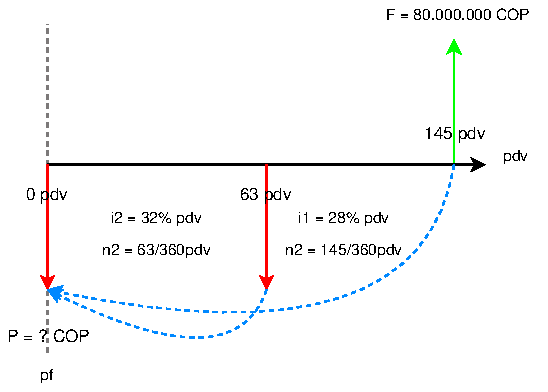
\includegraphics[trim=-78 -5 -78 -5]{3_Capitulo/img/ejemplos/11/capitulo3ejercicio11.pdf} }                                                                                         \\ \hline
			%%%%%%%%%%%%% FIN INSERCIÓN DE IMAGEN
			%%%%%FIN FLUJO DE CAJA
			
			
			
			%%%%% INICIO DECLARACIÓN FORMULAS
			%%%%%%%%%%% INICIO TITULO
			\rowcolor[HTML]{FFB183}
			\multicolumn{3}{|c|}{\cellcolor[HTML]{FFB183}\textbf{4. Declaración de fórmulas}}                                                                                    \\ \hline
			%%%%%%%%%%% FIN TITULO
			%%%%%%%%%%% INICIO MATEMÁTICAS
		
			 \multicolumn{3}{|c|}{$P=F(1+i    )^{-n}$\hspace{35pt}\textit{Valor presente}\hspace{0.3cm}}\\ \hline
			%%%%%%%%%% FIN MATEMÁTICAS
			%%%%%% INICIO DESARROLLO MATEMÁTICO
			\rowcolor[HTML]{FFB183}
			%%%%%%%%%%INICIO TITULO
			\multicolumn{3}{|c|}{\cellcolor[HTML]{FFB183}\textbf{5. Desarrollo matemático}}                                                                                      \\ \hline
			%%%%%%%%%% FIN TITULO
			%%%%%%%%%% INICIO MATEMÁTICAS
			\multicolumn{3}{|c|}{$Pc_1 =   80{.}000{.}000 COP (1+0,28)\frac{-145}{360}$ =   72{.}428{.}283,64 COP $\simeq$   72{.}428{.}284 COP \hspace{3pt}\textit{Ecuación de valor}}
			\\ 
			\multicolumn{3}{|c|}{$Pc_2 =   80{.}000{.}000 COP(1+0,32)\frac{-63}{360} =    76{.}206{.}067 COP$ \hspace{3pt}\textit{Ecuación de valor}}
			\\ 
			\multicolumn{3}{|c|}{$Pc_1 =  P_{C2} - P_{C1} COP  = 76{.}206{.}067 - 72{.}428{.}284  =   3{.}777{.}738 COP  $ \hspace{3pt}\textit{Ecuación de valor}}
			                             \\ \hline
			%%%%%%%%%% FIN MATEMÁTICAS
			%%%%%% FIN DESARROLLO MATEMÁTICO
			
			\rowcolor[HTML]{FFB183}
			\multicolumn{3}{|c|}{\cellcolor[HTML]{FFB183}\textbf{6. Respuesta}}    \\ \hline    
			
			\multicolumn{3}{|c|}{$P_{C2} - P_{C1} =  3{.}777{.}783 COP  $} \\ \hline
		\end{longtable}
		%Se crean dos lineas en blanco para que no quede el siguiente texto tan pegado
	\end{center}

%%%%%%%%%%%%%%%%%%%%%%%%%%FIN EJERCICIO X %%%%%%%%%%%%%%%%%%%%%%%%%%%
%\textbf{Ejemplo 9}\\
%Supongamos que un inversionista desea adquirir la aceptación bancaria del ejemplo anterior, la cual figura con una tasa de registro del 30\% periódico 40 días vencido y con precio de registro $P_{R} =  COP 97,165$ pero él también sabe que para adquirirla deberá pagar una comisión a un corredor de bolsa lo cual hará variar el precio que él debe pagar y también la rentabilidad que él pueda obtener.\\
%
%Supongamos que la comisión que cobra un corredor por la compra es del 0,475\% periodo 40 días periodo vencido\\
%¿Cuál es el precio del inversionista?$ P_{c} =  COP ? $, que incluye la comisión del comisionista vendedor, el precio de registro y la comisión de bolsa del comprador. El punto de referencia es el precio de registro $P_{R}$.\\
%¿Cuál es la rentabilidad del inversionista? $i_{c} = ? \%$ periódica 40 días vencido, o $j =? nadv$
%
%\textbf{Solución}\\
%\begin{itemize}
%  \item a. Diagrama de flujo\\
%        \begin{center}
%          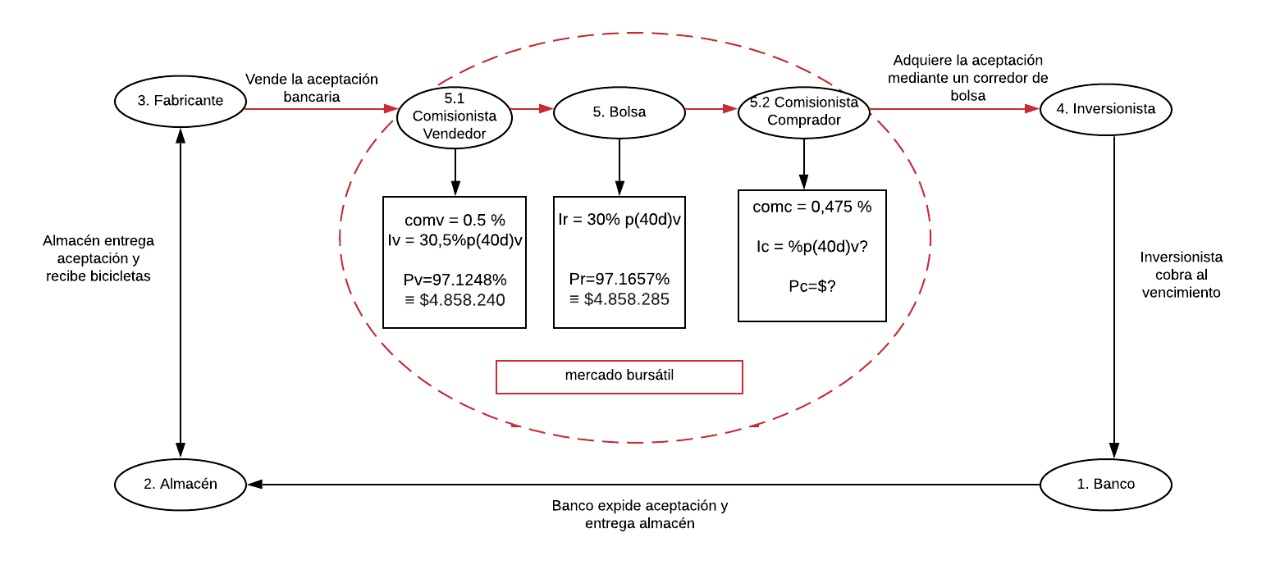
\includegraphics[height=6.0cm]{3_Capitulo/img/ejemplos/3_10}
%        \end{center}
%  \item b. Declaración de variables\\
%        $i_{c} = 30\% - 0,475\% = 29,525\% p 40dv\\
%          P_c =  COP ?$\\
%        $n= \frac{40}{365} p (40días) $\\
%        $P_{R}=?$\\
%  \item c.Declaración de formulas\\
%        \\
%        P = $F(1+i)^{n}$ \hspace{35pt}\textit{Valor presente}\\
%  \item d. Desarrollo matemático:\\
%        \\
%        $P_c =   COP 100(1+0,29525)^\frac{40}{365} =  COP 97,2047$ \hspace{35pt}\textit{Ecuación de valor} \\
%        $P_{R}$ =  COP 97,2047\% ( COP 5{.}000{.}000) =  COP 4{.}860,245\\
%        $P_c-P_{R}$ =  COP 4{.}860,235 -  COP 4{.}858,285 =  COP 1{.}950\\
%  \item e. Respuesta\\
%        \\
%        Precio del Inversionista =  COP  97,2047 y la rentabilidad inversionista fue de 29,52\% p(40dv) \\
%
%
%\end{itemize}
%\textbf{Observación:} En el mercado bursátil el precio del vendedor es diferente al precio del comprador debido a la comisión de los corredores de bolsa, pero en el mercado extrabursátil estos valores son iguales dado que no hay comisión.\\
%
%En el ejemplo anterior hemos mostrado el procedimiento de negociación en los mercados extra bursátil y bursátil, pero por simplicidad no hemos incluido el impuesto y la comisión que cobra el banco por la expedición de la aceptación bancaria. En el siguiente ejemplo incluiremos este factor.\\
%\textbf{Ejercicio 10}\\
%
%Supongamos que faltando 10 días para el vencimiento el inversionista del ejemplo anterior decide venderlo y para esta época se están negociando en Bolsa con una tasa del 28\% período 10 días vencido, por lo tanto la tasa de registro debe ser del 28\% período 10 días Vencido. \\
%Calcular: \\
%El precio de registro en bolsa. \\
%La retención en la fuente que debe reconocer al vendedor. \\
%La tasa del vendedor. \\
%El precio de vendedor. \\
%Valor de venta.  \\
%Tasa del comprador. \\
%Valor del comprador. \\
%\begin{itemize}
%  \item a.Diagrama de flujo:\\
%
%  \item b.Declaración de variables
%
%        F =  COP 100\\ i= 28\% p(10d)v  COP n= \frac{10}{365}$p(10d)v\\
%        Pr =  COP ?\\
%  \item d.Declaración de formulas:\
%
%        $P=F(1+i    )^{-n}$\hspace{35pt}\textit{Valor presente}\\
%
%  \item e. Desarrollo matemático
%
%        $P_{R}= COP 100 (1+0,28)^\frac{-10}{365}$ = 99,32595\% \hspace{35pt}\textit{Ecuación de valor}\\
%
%        En pesos el valor de registro será: 99,3595\% x  COP 5{.}000{.}000 =  COP 4{.}966,298\\
%        Por lo tanto, la retención en la fuente será RF = 0,07*( COP 5{.}000{.}000 -  COP 4{.}966,298) =  COP 2{.}359\\
%        Suponiendo que las comisiones de compra y venta sean c/u del 0,5\% en rentabilidad la tasa del vendedor viene a ser 28\% + 0,5\% = 28,5\% período 10 días vencido y el precio de venta será:
%        \begin{center}
%          $	P_{V} = 100(1+0,285)^\frac{-10}{365}$ = 99,3153\% equivalente a 99,3153\%(  COP 5{.}000{.}000) =  COP 4{.}965,765\\
%        \end{center}
%        Por lo tanto el vendedor además de recibir los  COP 4{.}965{.}765 también debe recibir lo correspondiente a la retención en la fuente ( COP 2,359), En consecuencia el vendedor recibirá:\\
%        \begin{center}
%          $P_{V}$ =  COP 4{.}966{.}830 +  COP 2{.}539 =  COP 4{.}969{.}189
%        \end{center}
%        Para el comprador se tiene:
%        \begin{center}
%          Tasa de compra ic = 28\% - 0,5\% = 27,5\% p10dv
%        \end{center}
%        Precio de compra:
%        \begin{center}
%          Pc = $100(1+0,275)^\frac{-10}{365}$ = 99,3366\% equivalente a 99,3366\% x  COP 5{.}000{.}000 =  COP 4{.}966{.}830
%        \end{center}
%        El total que debe pagar el comprador será el precio de compra más la parte de retención en la fuente que la Bolsa le devuelve al vendedor, esto es:
%        \begin{center}
%          Pc Neto= 	 COP 4{.}966{.}830 +  COP 2{.}359 =  COP 4{.}969{.}189
%        \end{center}
%  \item e. Respuesta\\
%        \textbf{Observación 1:} El primer inversionista pagó por retención en la fuente  COP 9{.}920 y le reintegraron  COP 2{.}359 esto significa que en total pagó:  COP 9{.}920- COP 2{.}359	=  COP 7{.}561 y el segundo inversionista pagó  COP 2{.}359\\
%        \textbf{Observación 2:} La constitución de aceptaciones no implica desembolsos de dinero en forma inmediata ni por parte de la entidad financiera ni por parte del comprador, salvo el IVA de la mercancía,  la comisión de intermediario financiero, lo demás es una obligación futura.\\
%        \textbf{Observación 3:} Si una aceptación no es cobrada al vencimiento, el emisor debe consignar el valor de esta en el Banco Agrario, sin embargo el emisor da un período de gracia antes de hacer la correspondiente consignación.
%\end{itemize}
%\medskip
%
%\textbf{Ejemplo 11}\\
%
%Una aceptación bancaria por  COP 80 millones con fecha de vencimiento el 17 de diciembre de 1999 es adquirida en 22 de julio de 1999 por un primer inversionista con una tasa del de 28\% período 28 días vencidos y es cedida a un segundo inversionista el 14 de octubre de 1999. Si el segundo inversionista desea ganarse el 32\% período días vencido utilice un año de 360 (año de 360 días) \\
%¿Cuál es la ganancia en pesos del primer inversionista? \\
%¿cuál es la rentabilidad periódica días vencido del primer inversionista? \\
%
%Si tomamos en cuenta que debemos usar un año de 360 días entonces los días que hay entre el 22 de julio y el 17 de diciembre son 145 que se calculan así: \\
%
%\begin{center}
%  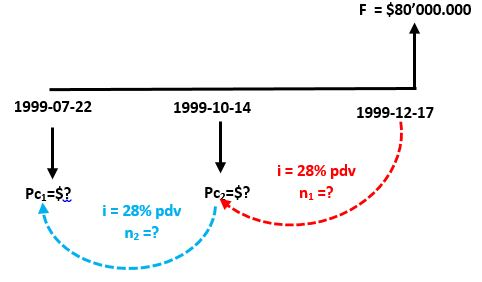
\includegraphics[height=5.0cm]{3_Capitulo/img/ejemplos/3_12}
%\end{center}
%
%Los días que hay entre el 14 de octubre y el 17 de diciembre se calculan así:
%
%
%\begin{center}
%  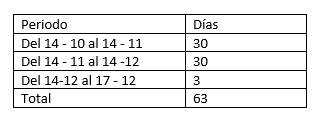
\includegraphics[height=3.0cm]{3_Capitulo/img/ejemplos/3_13}
%\end{center}
%
%\textbf{Solución}\\
%\begin{itemize}
%  \item a. Diagrama de flujo\\
%        \begin{center}
%          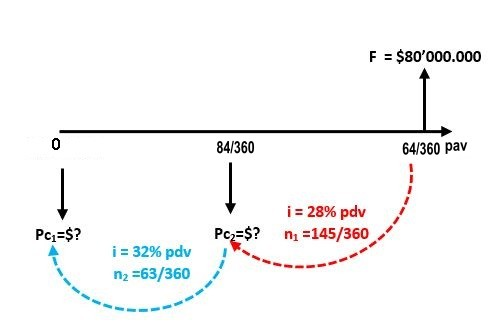
\includegraphics[height=4.0cm]{3_Capitulo/img/ejemplos/3_14}
%        \end{center}
%  \item b. Declaración de variables\\
%        $i_{1} = 28\% pav$ \\
%        $n_{1} = \frac{145}{360}$ pav\\
%        $i_{2} = 32 \%$ pdv\\
%        $n_{2} =\frac{63}{360}$pdv\\
%        $n_{3} = 145$ días - 63 días = 82 pdv.\\
%
%        $P_{c2}-P_{c1} = ?$\\\\
%
%  \item c. Declaración de formulas\\
%
%        P = $F(1+i)^{-n}$ \hspace{35pt}\textit{Valor presente}\\
%
%  \item d. Desarrollo matemático\\
%        $Pc_1 =  COP 80{.}000{.}000(1+0,28)\frac{-145}{360}$ =  COP  72{.}428{.}283,64 $\simeq$  COP 72{.}428{.}284 \hspace{35pt}\textit{Ecuación de valor}\\
%        $Pc_2 =  COP 80{.}000{.}000(1+0,32)\frac{-63}{360}$ =  COP  76{.}206{.}067,12\\
%  \item e. Respuesta:\\
%        La ganancia del primer inversionista será:\\
%        \begin{center}
%          $Pc_2 - Pc_1 =  COP 76{.}206{.}067 -  COP 72{.}428{.}284 =  COP 3{.}777{.}783$\\
%        \end{center}
%\end{itemize}
%En este caso el tiempo se puede hallar calculando los días que hay entre el 22 de julio y el 14 de octubre usando el procedimiento anterior, o, también por diferencia de días entre el total que es 145 y los que hay entre la fecha de compra del segundo inversionista y a la fecha de vencimiento que vienen a ser 63 días, entonces esta diferencia viene a ser: 145 - 63 = 82
%\begin{center}
%   COP 76{.}206{.}067 = $ COP 72{.}428{.}284(1+i)\frac{82}{360}$
%\end{center}
%De donde se obtiene que i= 25,01\%\ período 82 días vencidos \\
%La rentabilidad del segundo inversionista obviamente es del 32\% periodo (63 días vencidos).
%\chapter{Modelos de Conteo}

%\section{Introducción}\index{Introducción}



%----------------------------------------------------------------------------------------
%	PART
%----------------------------------------------------------------------------------------

%\part{Parte Dos}

%----------------------------------------------------------------------------------------
%	CHAPTER 3
%----------------------------------------------------------------------------------------

%\chapterimage{ima2} % Chapter heading image


%Anexos
%\chapter*{Anexos}
%\addcontentsline{toc}{chapter}{\textcolor{ocre}{Anexos}}




%----------------

%----------------------------------------------------------------------------------------
%	BIBLIOGRAPHY
%----------------------------------------------------------------------------------------

%\chapter*{Bibliografía}
%\addcontentsline{toc}{chapter}{\textcolor{ocre}{Bibliografía}}
%\section*{Books}
%\addcontentsline{toc}{section}{Books}
%\printbibliography[heading=bibempty,type=book]

%\begin{itemize}
%\item


%\end{itemize}


%----------------------------------------------------------------------------------------
%	INDEX
%----------------------------------------------------------------------------------------

\phantomsection
\setlength{\columnsep}{0.75cm}
\printindex
